\section{Application Implementation and Documentation}
\label{secD4:ApplicationImplementationAndDocumentation}
Nelle sezioni precedenti abbiamo individuato tutte le procedure e funzionalità che sono implementate nel prototipo del sito PlanIt e di come l'utente autenticato può utilizzarle nel suo flusso applicativo mostrando il diagramma "user flow". L'applicazione è stata sviluppata utilizzando NextJS (anche TypeScript ma solo in piccola parte per la documentazione) per la parte di API e FrontEnd, inoltre per la parte di UI (user interface) sono stati utilizzati anche CSS e React. Per la gestione dei dati abbiamo utilizzato MongoDB e la libreria mongoose. Per la gestione di autenticazione all'interno del sito abbiamo utilizzato il sistema esterno Auth0. Per la produzione della documentazione delle APIs abbiamo usato la libreria Swagger per NextJS, invece per il testing, sempre delle APIs, è stato usato il framework di JavaScript Jest. Infine, per fare le chiamate delle APIs da FrontEnd usiamo la libreria di JavaScript Axios.
\begin{listaPersonale} {APD}
    \elemento[Project Structure]{apd:ProjectStructure}
    La struttura del progetto è presentata nelle seguenti foto ed è composto da una cartella "api", dove sono presenti tutte le funzioni per la gestione delle APIs locali, divisi in base a quale struttura dati gestiscono (ovvero "event", "calendar", "user"), di una cartella "pages", al cui interno oltre che la cartella "api", sono presenti anche i file di estensione React indispensabili per comporre le interfacce grafiche di ciascuna schermata presente nel sito PlanIt, di una cartella "lib", in cui sono presenti i file usati per andare a stabilire la connessione con il database MongoDB, e, infine, di una cartella "models", dove ci sono i modelli di oggetti implementati per la gestione di dati del nostro sito. Si evidenzia che i modelli definiti sono presenti nel database MongoDB.\\
    Sottolineiamo che le uniche "pages" che sono state sviluppate in maniera completa sono "Calendario" e "Eventi". Evidenziamo che le varie componenti che vanno a comporre queste schermate sono state sviluppate in React nella cartella "components", che può essere sempre visualizzata nella seguente foto.\\
    Inoltre, nella cartella "styles" sono presenti i file "css" sviluppati per andare a definire i stili dei moduli presenti nell'interfaccia grafica, che saranno visualizzabili dall'utente che entra nel sito PlanIt.
    \begin{center}
        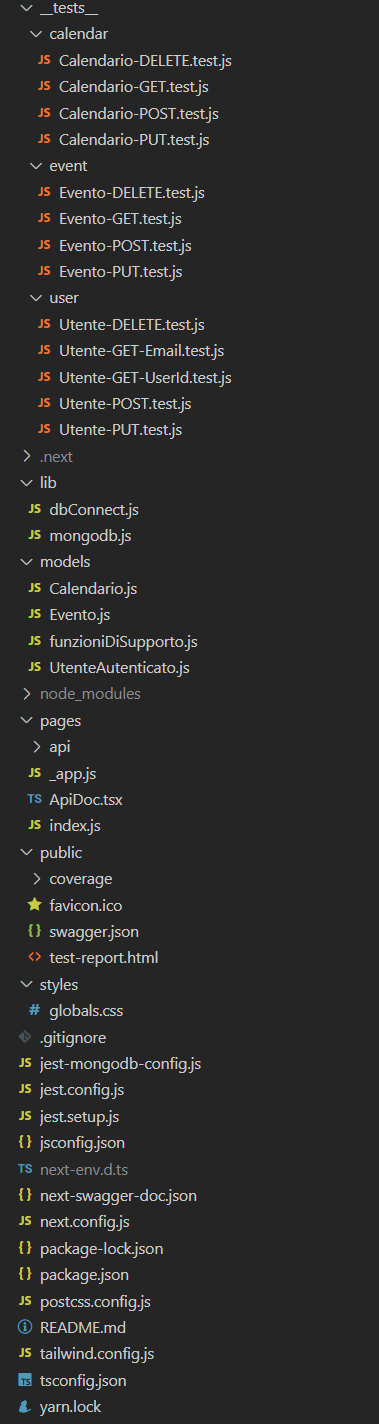
\includegraphics[width=0.27\textwidth, height=0.9\textheight]{img/png/project_structure/project_structure_totale.png}
        \blfootnote{Immagine \href{https://github.com/Life-planner/Documentazione/blob/main/D4/img/png/project_structure/project_structure_totale.png}{PNG} Struttura codice sorgente, 1a parte}
        \captionof{figure}{Struttura codice sorgente, 1a parte}
    \end{center}
    \begin{center}
        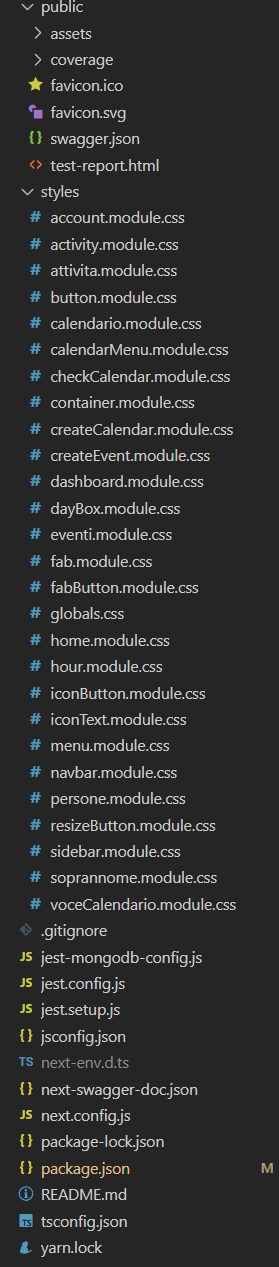
\includegraphics[width=0.3\textwidth, height=0.75\textheight]{img/png/project_structure/project_structure_totale_2.png}
        \blfootnote{Immagine \href{https://github.com/Life-planner/Documentazione/blob/main/D4/img/png/project_structure/project_structure_totale_2.png}{PNG} Struttura codice sorgente, 2a parte}
        \captionof{figure}{Struttura codice sorgente, 2a parte}
    \end{center}
    \newpage
    \elemento[Project Dependencies]{apd:ProjectDependencies}
    I seguenti moduli sono stati utilizzati e aggiunti al file "package.json", il cui contenuto è anche visualizzabile nella seguente foto:
    \begin{itemize}
        \item MongoDB, usato per fare il testing;
        \item Mongoose, libreria usata per connettersi al database MongoDB.
        \item NextJS, framework utilizzato per lo sviluppo delle APIs e del FrontEnd del sito PlanIt;
        \item Swagger, tool utilizzato per la documentazione delle APIs; la libreria "next-swagger-doc", da noi utilizzata, è semplicemente Swagger per Next.
        \item React, libreria di JavaScript per l'implementazione dell'UI del sito;
        \item Jest, framework di JavaScript utilizzato per andare a fare il testing delle APIs;
              \begin{comment}
              \item PostCSS, è uno strumento di sviluppo software che utilizza plug-in basati su JavaScript per automatizzare le operazioni CSS di routine e quindi lo sviluppo dei moduli presenti nel FrontEnd del nostro sito;
              \end{comment}
        \item TypeScript, estensione di JavaScript, usata solo in minima parte nello sviluppo delle APIs, ovvero nello sviluppo degli esempi per la documentazione di queste.
        \item Axios, libreria di JavaScript che permette da FrontEnd di connettersi con le API di backend e gestire le richieste effettuate tramite il protocollo HTTP.
        \item Toastify, libreria di React che permette di fare dei pop-up di "notifacation"; pop-up di "notification" che utilizzeremo nel FrontEnd.
    \end{itemize}
    \begin{center}
        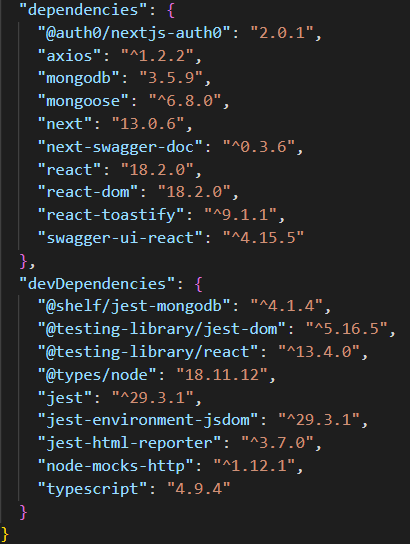
\includegraphics[width=0.47\textwidth, height=0.45\textheight]{img/png/package_json.png}
        \blfootnote{Immagine \href{https://github.com/Life-planner/Documentazione/blob/main/D4/img/png/package_json.png}{PNG} Project Dependencies}
        \captionof{figure}{Project Dependencies}
    \end{center}
    \newpage
    \elemento[Project Data or DB]{apd:ProjectDB}
    Per la gestione dei dati utili all'applicazione abbiamo definito tre principali strutture dati, come illustrato nelle seguenti immagini. Infatti, le strutture dati che abbiamo deciso di avere in questo prototipo del nostro sito PlanIt, sono:
    \begin{itemize}
        \item "UtenteAutenticato", struttura dati che individua l'utente che si è autenticato ed accede al sito;
        \item "Evento", componente fondamentale del calendario, che sta alla base della logica del nostro sito ideato.
        \item "Calendario", contenitore di eventi, struttura dati sopra citata.
    \end{itemize}
    \begin{center}
        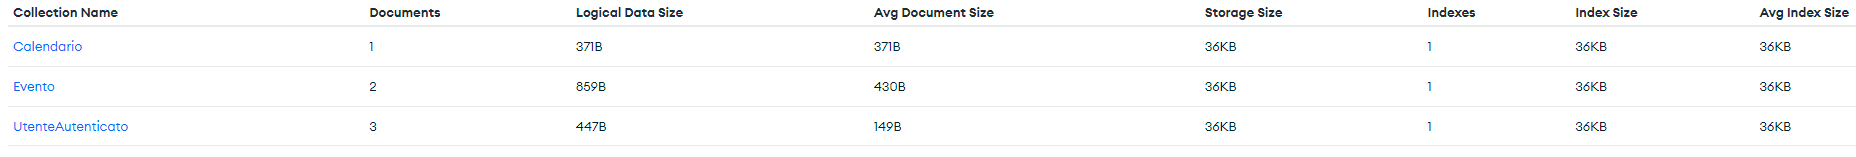
\includegraphics[width=1.1\textwidth, height=0.07\textheight]{img/png/DB/collections.png}
        \captionof{figure}{Collections delle strutture dati usate nell'applicazione}
        \blfootnote{Immagine \href{https://github.com/Life-planner/Documentazione/blob/main/D4/img/png/DB/collections.png}{PNG} Collections}
    \end{center}
    \begin{center}
        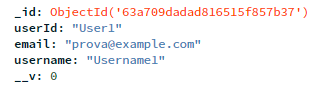
\includegraphics[width=0.45\textwidth, height=0.1\textheight]{img/png/DB/utente_autenticato.png}
        \captionof{figure}{Tipo di dato "Utente Autenticato"}
        \blfootnote{Immagine \href{https://github.com/Life-planner/Documentazione/blob/main/D4/img/png/DB/utente_autenticato.png}{PNG} Tipo di dato "Utente Autenticato"}
    \end{center}
    \begin{center}
        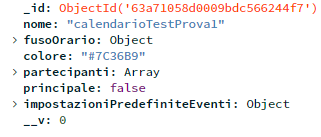
\includegraphics[width=0.5\textwidth, height=0.15\textheight]{img/png/DB/calendario.png}
        \captionof{figure}{Tipo di dato "Calendario"}
        \blfootnote{Immagine \href{https://github.com/Life-planner/Documentazione/blob/main/D4/img/png/DB/calendario.png}{PNG} Tipo di dato "Calendario"}
    \end{center}
    \begin{center}
        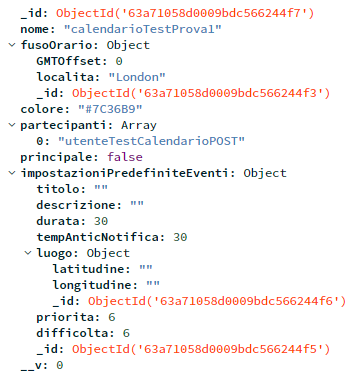
\includegraphics[width=0.55\textwidth, height=0.4\textheight]{img/png/DB/calendario_intero.png}
        \captionof{figure}{Tipo di dato "Calendario" con gli oggetti contenuti "esplorati"}
        \blfootnote{Immagine \href{https://github.com/Life-planner/Documentazione/blob/main/D4/img/png/DB/calendario_intero.png}{PNG} Tipo di dato "Calendario" con gli oggetti contenuti "esplorati"}
    \end{center}
    \begin{center}
        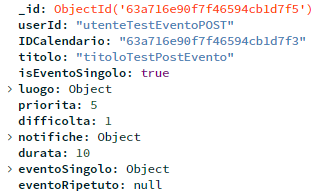
\includegraphics[width=0.55\textwidth, height=0.25\textheight]{img/png/DB/evento_singolo.png}
        \captionof{figure}{Tipo di dato "Evento", in questo caso è un evento singolo, che quindi è presente solo in un giorno specifico}
        \blfootnote{Immagine \href{https://github.com/Life-planner/Documentazione/blob/main/D4/img/png/DB/evento_singolo.png}{PNG} Tipo di dato "Evento" singolo}
    \end{center}
    \begin{center}
        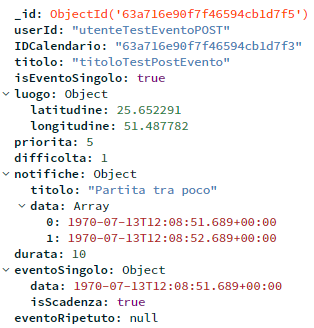
\includegraphics[width=0.45\textwidth, height=0.35\textheight]{img/png/DB/evento_singolo_intero.png}
        \captionof{figure}{Tipo di dato "Evento" singolo con gli oggetti contenuti "esplorati"}
        \blfootnote{Immagine \href{https://github.com/Life-planner/Documentazione/blob/main/D4/img/png/DB/evento_singolo_intero.png}{PNG} Tipo di dato "Evento" singolo con gli oggetti contenuti "esplorati"}
    \end{center}
    \begin{center}
        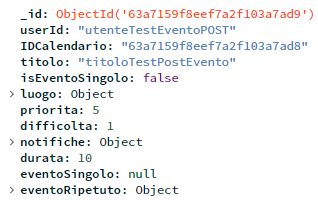
\includegraphics[width=0.5\textwidth, height=0.25\textheight]{img/png/DB/evento_ripetuto.png}
        \captionof{figure}{Tipo di dato "Evento", in questo caso è un evento ripetuto, che quindi è presente su più giorni}
        \blfootnote{Immagine \href{https://github.com/Life-planner/Documentazione/blob/main/D4/img/png/DB/evento_ripetuto.png}{PNG} Tipo di dato "Evento" ripetuto}
    \end{center}
    \begin{center}
        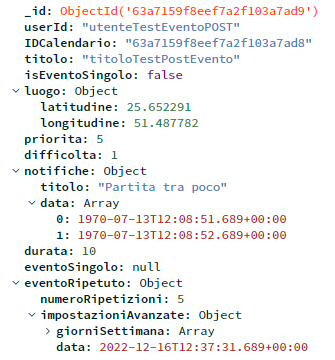
\includegraphics[width=0.5\textwidth, height=0.4\textheight]{img/png/DB/evento_ripetuto_intero.png}
        \captionof{figure}{Tipo di dato "Evento" ripetuto con gli oggetti contenuti "esplorati"}
        \blfootnote{Immagine \href{https://github.com/Life-planner/Documentazione/blob/main/D4/img/png/DB/evento_ripetuto_intero.png}{PNG} Tipo di dato "Evento" ripetuto con gli oggetti contenuti "esplorati"}
    \end{center}
    \newpage
    \elemento[Project APIs]{apd:ProjectAPIs}
    In questo capitolo, verranno presentate le APIs che sono state sviluppate in questo prototipo del sito PlanIt. Infatti, si passerà dall'esposizione dell' Extract Diagram, diagramma che serve come collegamento tra il Class Diagram alla APIs, e Resources Models, diagramma in cui sono presenti tutte le risorse implementate, alla descrizione del vero e proprio codice delle APIs, presentati in questi primi diagrammi.
    \begin{listaPersonale2}[APD]{}
        \elemento[Resources Extraction from the Class Diagram]{apd:ResourceExtraction}
        Questo diagramma si può dire che faccia da vero e proprio "ponte" tra Class Diagram, presentato nel documento D3, e le resources che andremo ad implementare con le nostre APIs. \\
        Come si può notare, abbiamo individuato dodici resources che riteniamo fondamentali per sviluppare la logica che sta alla base del nostro sito PlanIt. \\
        \begin{itemize}
            \item Partendo dalla classe "UtenteAutenticato", presentata in \prettyref{D3-dcl:TipologieUtenti}, abbiamo individuato tre resources, ovvero:
                  \begin{itemize}
                      \item CreaAccount, di tipo POST. Risorsa che ha lo scopo di creare un account all'interno del database MongoDB e per questo motivo ha l'etichetta "BackEnd"; infatti l'effetto principale di questa API avviene nel "BackEnd" con la creazione dell'account nel database.\\ L'account è una struttura dati già presentata nel capitolo precedente, ovvero "UtenteAutenticato", e l'input delineato è un "body" in quanto è formato da più di tre parametri, i quali verranno specificati e descritti nel diagramma Resources Model, presentato nel successivo capitolo.
                      \item ModificaAccount, di tipo PUT. Risorsa che ha il fine di dare la possibilità di andare a modificare un account già presente nel nostro database. L'etichetta "BackEnd" e l'input body sono presenti per gli stessi motivi definiti per la resource "CreaAccount".
                      \item GetDatiAccount, di tipo GET. API che ha lo scopo di ottenere i dati di un "UtenteAutenticato" conoscendo l'userId di tale utente. L'effetto ultima di questa resource è nel FrontEnd, in quanto i dati appariranno all'utente e quindi si è deciso di mettere come sua etichetta "FrontEnd"
                      \item GetDatiAccount\_email, di tipo GET. Risorsa analoga a quella precedente, con la sola differenza che l'account, da cui estrarre i dati, non è definito mediante l' "userId", "id" e stringa che identifica univocamente un utente, ma mediante la sua email che ha utilizzato per registrarsi.
                  \end{itemize}
            \item Dopo abbiamo individuato altre tre resources, partendo dalla classe "Evento", già presentata in \prettyref{D3-dcl:CreazioneModificaEvento}, ovvero:
                  \begin{itemize}
                      \item creaEvento, di tipo POST. Resource che ha lo scopo di andare a creare un evento che viene salvato nel database MongoDB. L'input che viene preso da questa API è un insieme di parametri che vanno a formare un oggetto di tipo "Evento", struttura dati già definita nel capitolo precedente, che in quanto piuttosto complicata, non siamo andati a specificare in questo diagramma ma nel "Resources Model" e qua ci siamo fermati nel scrivere come input solo "body". In quanto ha un effetto sul "BackEnd", con il salvataggio dell'evento nel database, abbiamo indicato come etichetta "BackEnd".
                      \item modificaEvento, di tipo PUT; grazie alla sua esecuzione abbiamo la modifica di un determinato evento già presente nel database appartenente ad un utente. In quanto ha un effetto finale nel database, gli abbiamo attribuito l'etichetta "BackEnd".
                      \item eliminaEvento, di tipo DELETE. Lo scopo di questa resource è quello di dare la possibilità di eliminare un "Evento" dato il suo "IDEvento" e l'"userId" dell'utente autenticato che ha questo determinato "Evento" che vuole eliminare. In quanto ha un effetto finale nel database, gli abbiamo attribuito l'etichetta "BackEnd".
                      \item getEventi, di tipo GET. Risorsa mediante cui si ottengo gli eventi di un calendario, dato l'"userId" dell'utente che ha tale calendario e l' "IDCalendario" del calendario da cui vogliamo estrarre gli eventi. L'etichetta "FrontEnd" è stata messa in quanto questa API è fondamentale per mostrare all'utente finale nell'user interface gli eventi di un determinato calendario.
                  \end{itemize}
                  Si specifica che tutte le resources individuate riguardano a funzioni già presentate in \prettyref{D3-dcl:CreazioneModificaEvento}.
            \item Infine abbiamo sviluppato tre resources per la classe "Calendario", tipo di dato già presentato nel precedente capitolo, le cui funzionalità e attributi sono stati descritti in \prettyref{D3-dcl:CreazioneModificaCalendario}. Le tre resources sono:
                  \begin{itemize}
                      \item creaCalendario, di tipo POST. API che ha lo scopo di creare un calendario all'interno del database MongoDB, e per questo motivo ha come etichetta "BackEnd". In quanto, per andare a creare un "Calendario" all'interno del database servono gli attributi che formano un oggetto di tipo "Calendario" e l' "userId" dell'utente che vuole creare tale calendario, come input abbiamo indicato body. L'input verrà descritto maggiormente nel Resources Model che viene presentato nel successivo capitolo.
                      \item modificaCalendario, di tipo PUT; grazie alla sua esecuzione abbiamo la modifica di un determinato calendario già presente nel database appartenente ad un utente. In quanto ha un effetto finale nel database, gli abbiamo attribuito l'etichetta "BackEnd".
                      \item eliminaCalendario, di tipo DELETE. Lo scopo di questa resource è quello di dare la possibilità di eliminare un "Calendario" dato il suo "IDCalendario" e l'"userId" dell'utente autenticato che ha questo determinato "Calendario" che vuole eliminare. In quanto ha un effetto finale nel database, gli abbiamo attribuito l'etichetta "BackEnd".
                      \item getCalendari, di tipo GET. API che ha lo scopo di ottenere tutti i calendari di un determinato "UtenteAutenticato", dato il suo "userId". Questa risorsa è fondamentale per andare a mostrare i calendari appartenenti all'utente, che potrà, quindi, visualizzare.
                  \end{itemize}
                  Si specifica che tutte le resources individuate riguardano a funzioni già presentate in \prettyref{D3-dcl:CreazioneModificaCalendario}.
        \end{itemize}

        \begin{center}
            \includesvg[width=1\textwidth, height=1\textheight]{img/svg/diagrammi/UML_API_diagram.svg}
            \blfootnote{Immagine \href{https://github.com/Life-planner/Documentazione/blob/main/D4/img/png/diagrammi/UML_API_diagram.png}{PNG}/\href{https://github.com/Life-planner/Documentazione/blob/main/D4/img/svg/diagrammi/UML_API_diagram.svg}{SVG} Extract Diagram}
        \end{center}
        \newpage


        \elemento[Resources Models]{apd:ResourcesModel}
        La seguente immagine mostra tutte le resources sviluppate nel nostro prototipo del sito PlanIt che sono state già presentate in parte nel precedente capitolo (\ref{apd:ResourceExtraction}), ma in questo capitolo, e nelle seguenti figure, si va più nello specifico di come funzionano queste APIs, andando a specificare in maniera dettagliata gli input e gli output possibili di ciascuna risorsa. \\
        Abbiamo deciso di non presentare solo il diagramma totale di tutti i resources models, ovvero quello successivo, ma anche altri tre diagrammi, con lo scopo di far visualizzare con più facilità tutte le risorse; infatti, si è andato a suddividere le resources presenti nel diagramma totale. Infatti in questi tre diagrammi sono presenti le resources, già presenti in quello totale, ma divise nei tre diversi diagrammi in base a come sono state già divise nell' Extract Diagram (\ref{apd:ResourceExtraction}).
        C'è una cosa comune che si può notare prima di andare nel dettaglio della descrizione di ciascuna risorsa, ovvero che praticamente tutte le risorse danno le stesse possibile risposte/output, che sono:
        \begin{itemize}
            \item 200 OK. Serve ad indicare che la procedura effettuata dall'API è andata a buon fine e l'esecuzione è avvenuta con successo. Infatti "200 OK" è la risposta standard per le richieste HTTP andate a buon fine.
            \item 400 BAD REQUEST. Serve ad indicare che la richiesta non può essere soddisfatta a causa di errori di sintassi, quindi abbiamo ottenuto un errore dall'esecuzione dell' API. Per errori di sintassi si intendono errori che riguardano soprattutto l'input inserito, il quale ha un formato sbagliato e quindi la procedura che deve effettuare l'API non può andare a buon fine e si riceve un messaggio di errore accompagnato dal codice "400". Oppure, non si sono inseriti tutti i parametri necessari affinché l'API possa funzionare e quindi riceviamo sempre questo codice "400" con un messaggio di errore.
            \item 409 CONFLICT. Serve ad indicare che la richiesta non può essere portata a termine a causa di un conflitto con lo stato attuale della risorsa. Un caso che potrebbe portare ad un conflitto è ad esempio l'invio di un dato in input che è un duplicato di un dato già presente nel database, come un evento, calendario ed utente. Gli eventi, calendari e utenti duplicati inviati in input non possono essere creati e messi nel database, in quanto c'è il dato duplicato che crea conflitto. Questo errore lo otteniamo anche quando un determinato dato che stiamo passando non è presente nel database o non appartiene all'utente che lo sta inviando, questo può essere il caso in cui l' "userId" di un utente non esiste, oppure il "Calendario" o "Evento" passati con il loro "id" non appartengono a quell'utente identificato dall' "userId" inviato.
            \item 500 INTERNAL SERVER ERROR. Serve ad indicare un errore che riguarda il server interno. Questo errore non ha fatto andare a buon fine l'esecuzione dell' API, come ad esempio la sconnessione dal database MongoDB, dove sono inseriti i vari oggetti che vengono salvati.
            \item 501 NOT IMPLEMENTED. Questo errore indica che non si è stati in grado di soddisfare il metodo della richiesta. Quindi si può descrivere come un errore generico, che non specifica nessun dettaglio sul perché non sia andata a buon fine l'esecuzione dell' API.
        \end{itemize}
        Si specifica che da questo momento in poi, verranno scritti assieme i codici di risultato con i messaggi di risposta per pura comodità. Infatti invece che scrivere "Tale API invia "400" come codice di risposta e messaggio di errore "Wrong format for (something)", verrà scritto direttamente "Tale API invia come messaggio di errore "400 - Wrong format for (something)" ".
        \begin{center}
            \includesvg[width=1\textwidth, height=1\textheight]{img/svg/diagrammi/Resources_Model.svg}
            \captionof{figure}{Resources Model completo}
            \blfootnote{Immagine \href{https://github.com/Life-planner/Documentazione/blob/main/D4/img/png/diagrammi/Resources_Model.png}{PNG}/\href{https://github.com/Life-planner/Documentazione/blob/main/D4/img/svg/diagrammi/Resources_Model.svg}{SVG} Resources Model completo}
        \end{center}
        \newpage
        \begin{listaPersonale3}[APD]{}
            \elemento[Resource Models "Calendario"]{apd:ResourcesModelCalendario}
            Nel seguente diagramma vengono presentate le APIs che riguardano la struttura dati "Calendario"; le risorse individuate per questa struttura dati, sono:
            \begin{itemize}
                \item "Elimina Calendario", resource di tipo DELETE. Questa API, già descritta in \ref{apd:ResourceExtraction}, ha la funzione di eliminare un calendario specifico, dato il suo "IDCalendario" e l' "userId" dell'utente autenticato che vuole eliminare quel determinato calendario. Gli output sono quelli già descritti in precedenza, ma specifichiamo quali sono i casi in cui si ottiene l'errore "400". Otteniamo questo errore di risposta, quando manca un parametro (messaggio di errore "Parameter missing"), ovvero o "userId" o "IDCalendario". Invece, l'errore "409" si ottiene quando l' "userId" è un duplicato (messaggio di errore "There are too many users with that userId" ) o non esiste (messaggio di errore "There is no user with that userId") o l' "IDCalendario", del calendario che si vuole eliminare, non appartiene alla lista di calendari di quell'utente specificato con l' "userId" (messaggio di errore "You do not own the calendar").
                \item "Modifica Calendario", resource di tipo PUT. Questa API, già descritta in parte in \ref{apd:ResourceExtraction}, ha la funzione di modificare un determinato calendario, dati tutti gli attributi che definiscono questa struttura dati modificata, e l' "userId" dell'utente che vuole modificare tale calendario. Specifichiamo, che si ottiene l'errore "400" ogniqualvolta non si è inserito uno degli attributi della struttura dati "Calendario", che si possono osservare nell'oggetto "Calendario" in input a questa API, con il messaggio "Parameter missing". \\
                      Infine, questa resource ha anche gli errori che verranno specificati nella descrizione di "Crea Calendario", descritta qua sotto.
                \item "Crea Calendario", resource di tipo POST. Questa API, già descritta in parte in \ref{apd:ResourceExtraction}, ha la funzione di creare e salvare nel database MongoDB il calendario formato dai parametri inviati in input per l'utente specificato con il parametro "userId". A differenza della resource PUT per il calendario, questa può avere anche dei campi vuoti in input senza che si ottenga un errore, ovvero questi campi: "fusoOrario", "colore", "principale" e "GestioneImpostazioniPredefiniteEventi". Invece i parametri "nome" e "userId" devono essere per forza non vuoti. Però, è da specificare che dagli attributi "fusoOrario", "colore" e "principali" si possono ottenere altri errori, ovvero:
                      \begin{itemize}
                          \item errore "400" nel caso in cui il colore inserito avesse un formato sbagliato ("400" con messaggio di errore "Wrong format for color");
                          \item errore "400" nel caso in cui il fusoOrario inserito avesse un formato sbagliato; infatti "GMTOffset" deve stare tra -12 e +12 e l'attributo "localita" deve essere diverso da "null". Se così non fosse riceviamo il codice "400" con messaggio di errore "Wrong format for fusoOrario";
                          \item errore "409" nel caso in cui principale fosse uguale a "true", ovvero stiamo creando il calendario principale di un utente, e l'utente, specificato dall' "userId" inserito, avesse già un calendario principale. Infatti non si possono avere più di un calendario principale, quindi otteniamo come risposta: "409 - There are too many primary calendars";
                      \end{itemize}
                      Infine, l'errore "409" si potrebbe ottenere anche quando l' "userId" dell'utente, che sta creando il calendario, è un duplicato o non esiste nel database. Si ottiene come messaggio di errore: "There are too many users with that userId" o "There is no user with that userId" rispettivamente.
                \item "Get Calendari", resource di tipo GET. Resource che ha lo scopo di ottenere tutti i calendari appartenenti ad un utente, dato il suo "userId": questo, ovviamente, deve essere non vuoto per non ricevere il messaggio di errore "400 - Parameter missing". Inoltre, nel caso in cui passassimo l' "userId" di un utente autenticato che non ha calendari, otteniamo il codice "409" con il messaggio di errore "There are no calendars with that userId". Gli altri errori e messaggi che si possono ricevere sono gli stessi già descritti in generale all'inizio del capitolo.
            \end{itemize}
            \begin{center}
                \includesvg[width=1\textwidth, height=1\textheight]{img/svg/diagrammi/Resources_Model_calendar.svg}
                \captionof{figure}{Resources Model riguardo solo il "Calendario"}
                \blfootnote{Immagine \href{https://github.com/Life-planner/Documentazione/blob/main/D4/img/png/diagrammi/Resources_Model_calendar.png}{PNG}/\href{https://github.com/Life-planner/Documentazione/blob/main/D4/img/svg/diagrammi/Resources_Model_calendar.svg}{SVG} Resources Model riguardo solo il "Calendario"}
            \end{center}
            \elemento[Resource Models "Evento"]{apd:ResourcesModelEvento}
            Nel seguente diagramma vengono mostrate le APIs che riguardano la struttura dati "Evento", già presentate in parte in \ref{apd:ResourceExtraction}; le APIs individuate per "Evento" sono:
            \begin{itemize}
                \item "Crea Evento", resource di tipo POST. Questa API ha lo scopo di andare a salvare un evento nel database usando i parametri dati in input. Gli output sono sempre quelli citati in generale in precedenza, ma si specifica che i parametri obbligatori, per non ottenere l'errore "400 - IDCalendario or titolo or evento details missing", sono: "IDCalendario", id del calendario in cui stiamo aggiungendo questo evento, "titolo", titolo dell'evento, "userId", id dell'utente che sta creando l'evento, "isEventoSingolo", booleano che indica se l'evento che si sta creando è un evento singolo o ripetuto. Inoltre se "isEventoSingolo" è uguale a true si deve avere anche l'oggetto "eventoSingolo" diverso da "null", invece se questo è uguale a false, "eventoRipetuto" deve essere diverso da "null".
                \item "Modifica Evento", resource di tipo PUT. Questa resource ha lo scopo di andare a modificare un evento specifico appartenente ad un utente autenticato. A differenza dell' API "Crea Evento", questa API ha bisogno di tutti gli attributi che costituiscono la struttura dati "Evento" eccetto "eventoSingolo" o "eventoRipetuto", che possono essere uguali a "null", a seconda del valore del booleano isEventoSingolo, per i casi già citati per "Crea Evento". Dunque per non ricevere l'errore "400 - Parameter missing", questa resource ha bisogno di tutti gli attributi facenti parte di "Evento", che si possono osservare nel diagramma successivo in \ref{apd:ProjectDB}. Gli altri errori che si possono ottenere da questa resource sono gli stessi già citati in precedenza in generale; ovviamente visto che i parametri da inserire obbligatoriamente sono di più, è più facile che si possa sbagliare e ottenere l'errore "400 - Wrong format for (inserted parameter uncorrectly)".
                \item "Elimina Evento", resource di tipo DELETE. Questa API ha lo scopo di eliminare un specifico evento di un utente autenticato, per questo motivo i parametri necessari sono: "IDEvento", "id" dell'evento che si vuole eliminare, e "userId", "id" dell'utente autenticato che vuole eliminare un suo evento. Se manca uno dei due parametri, ovviamente si ottiene l'errore "400 - Parameter missing". Gli altri output che si possono ottenere da questa API, sono quelli già descritti nella lista di possibile risposte di ciascuna API, con particolare attenzione al caso in cui viene inviato l' "IDEvento" di un evento che non appartiene a quel dato "userId"; in questo caso, si riceve l'errore "400 - You do not own the event".
                \item "Get Eventi", resource di tipo GET. API che ha la funzione di ritornare tutti gli eventi di un dato calendario. I parametri necessari, affinché questa resource possa effettuare il suo lavoro, sono l' "IDCalendario", "id" del calendario di cui vogliamo ottenere gli eventi, e l' "userId" dell'utente che ha tale calendario. Questi devono essere diversi da "null" per non ricevere il messaggio di errore "400 - Parameter missing". Inoltre, nel caso in cui passassimo l' "IDCalendario" di un calendario vuoto, ovvero senza eventi, viene ritornato il codice "409" con il messaggio di errore "There are no events with that userId and IDCalendario". Gli altri errori e messaggi che si possono ricevere sono gli stessi già descritti in generale all'inizio del capitolo.
            \end{itemize}
            \begin{center}
                \includesvg[width=1\textwidth, height=1\textheight]{img/svg/diagrammi/Resources_Model_event.svg}
                \captionof{figure}{Resources Model riguardo solo l' "Evento"}
                \blfootnote{Immagine \href{https://github.com/Life-planner/Documentazione/blob/main/D4/img/png/diagrammi/Resources_Model_event.png}{PNG}/\href{https://github.com/Life-planner/Documentazione/blob/main/D4/img/svg/diagrammi/Resources_Model_event.svg}{SVG} Resources Model riguardo solo l' "Evento"}
            \end{center}
            \elemento[Resource Models "UtenteAutenticato"]{apd:ResourcesModelUtenteAutenticato}
            Nel seguente diagramma vengono mostrate le APIs che riguardano la classe "UtenteAutenticato", già presentate in parte in \ref{apd:ResourceExtraction}; le APIs individuate per "UtenteAutenticato" sono:
            \begin{itemize}
                \item "Modifica Account", resource di tipo PUT. La funzione di questa API è di modificare l' "username" di un utente autenticato, dato il suo "userId" e il nuovo "username"; ovviamente, per effettuare tale azione e non riceve il messaggio di errore "400 - Parameter missing", i parametri sopra citati devono essere sempre presenti. Gli altri errori che si possono riscontrare sono sempre i soliti presentati in generale all'inizio di questo capitolo.
                \item "Crea Account", resource di tipo POST. Lo scopo di questa resource è quella di creare un account all'interno del database, dato l' "email", l' "username" e l' "userId" dell'utente autenticato che si vuole creare; è importante specificare che tutti questi tre parametri devono essere diversi da "null" per non ottenere il messaggio di errore "400 - Parameter missing". Gli altri errori e risposte che si possono riscontrare sono gli stessi già citati in generale all'inizio del paragrafo.
                \item "Get Dati Utente" e "Get Dati Utente\_email", APIs di tipo GET. Si descrivono assieme queste APIs, in quanto hanno la stessa funzione, ovvero ottenere i dati dell'account di un utente ("email", "userId", "username"), ma dando parametri diversi: per "Get Dati Utente" basta inviare l' "userId" dell'utente autenticato, invece per "Get Dati Utente\_email" basta la propria "email". Si è deciso di mettere entrambi i GET, in quanto entrambi gli attributi "email" e "userId" dovrebbero univoci per ciascun utente autenticato. Ovviamente, per non ottenere il messaggio di errore "400 - Parameter missing", il parametro che deve essere sempre presente e diverso da "null" è l' "userId" o l' "email" rispettivamente. Gli altri errori e messaggi che si possono ricevere sono gli stessi già descritti in generale all'inizio del paragrafo.
            \end{itemize}
            \begin{center}
                \includesvg[width=0.9\textwidth, height=1\textheight]{img/svg/diagrammi/Resources_Model_GestioneChiamateMongoDB.svg}
                \captionof{figure}{Resources Model riguardo solo "UtenteAutenticato"}
                \blfootnote{Immagine \href{https://github.com/Life-planner/Documentazione/blob/main/D4/img/png/diagrammi/Resources_Model_GestioneChiamateMongoDB.png}{PNG}/\href{https://github.com/Life-planner/Documentazione/blob/main/D4/img/svg/diagrammi/Resources_Model_GestioneChiamateMongoDB.svg}{SVG} Resources Model riguardo solo "UtenteAutenticato"}
            \end{center}
        \end{listaPersonale3}
    \end{listaPersonale2}
    \elemento[Sviluppo API]{apd:SviluppoAPI}
    In questo capitolo verranno presentate le API delle resources già sopra descritte, però andando più nello specifico mostrando il codice di come queste resources sono state implementate.
    \begin{listaPersonale2}[APD]{}
        \elemento [Crea Calendario] {apd:creaCalendario}
                Mediante questa API, l'applicativo salva nel database MongoDB un calendario con gli attributi uguali ai parametri ricevuti in input, per l'utente autenticato identificato dal suo "userId", parametro preso in input da questa funzione.
                Come già detto in precedenza nella descrizione della resource corrispondente in \ref{apd:ResourcesModelCalendario}, nel caso in cui mancasse l'attributo "nome" o l' "userId" non sarebbe possibile creare un calendario e quindi l'API manderebbe come messaggio di risposta il seguente errore: "400 - Name missing". Inoltre, come già detto in \ref{apd:ResourcesModelCalendario}, questa API controlla che il "colore" e "fusoOrario" inseriti rispettino degli standard affinché siano ritenuti accettabili: in caso non li rispettassero, riceveremmo rispettivamente i seguenti errori: "400 - Wrong format for color", "400 - Wrong format for fusoOrario". \\
                Mediante la funzione "find()", l' API va a cercare nel database, gli utenti autenticati che hanno l' "userId" inserito; nel caso in cui trovasse più di un utente con questo "userId", si riceve un messaggio di errore del tipo "400 - There are too many users with that userId"; invece, nel caso in cui trovasse nessun utente autenticato con tale "userId" si riceve il messaggio di errore "400 - There is no user with that userId". \\
                Infine, l'ultimo controllo, che si fa sugli attributi ricevuti in input, riguarda l'attributo "principale", booleano che indica se il calendario che si sta creando sia quello principale o meno. Infatti, ogni utente autenticato può avere al massimo un calendario principale, per questo motivo nel caso in cui si provasse a creare un calendario principale già esistente per quell' "userId", si riceve il messaggio di errore: "409 - There are too many primary calendars". \\
                Grazie, alla funzione "create()", viene creato nel database un calendario con i valori dei campi che lo formano uguali ai parametri inseriti in input; nel caso ci fossero degli errori nell'esecuzione di questa funzione, otteniamo l'errore "500 - Not inserted". Se, invece l'esecuzione di questa funzione è andata a buon fine, otteniamo il messaggio di successo "200 - Calendar inserted correctly". C'è un eventuale altro controllo che serve per individuare errori generici durante l'esecuzione di creaCalendario, quindi otteniamo un messaggio di errore del tipo: "501 - Generic error".
                \begin{center}
                    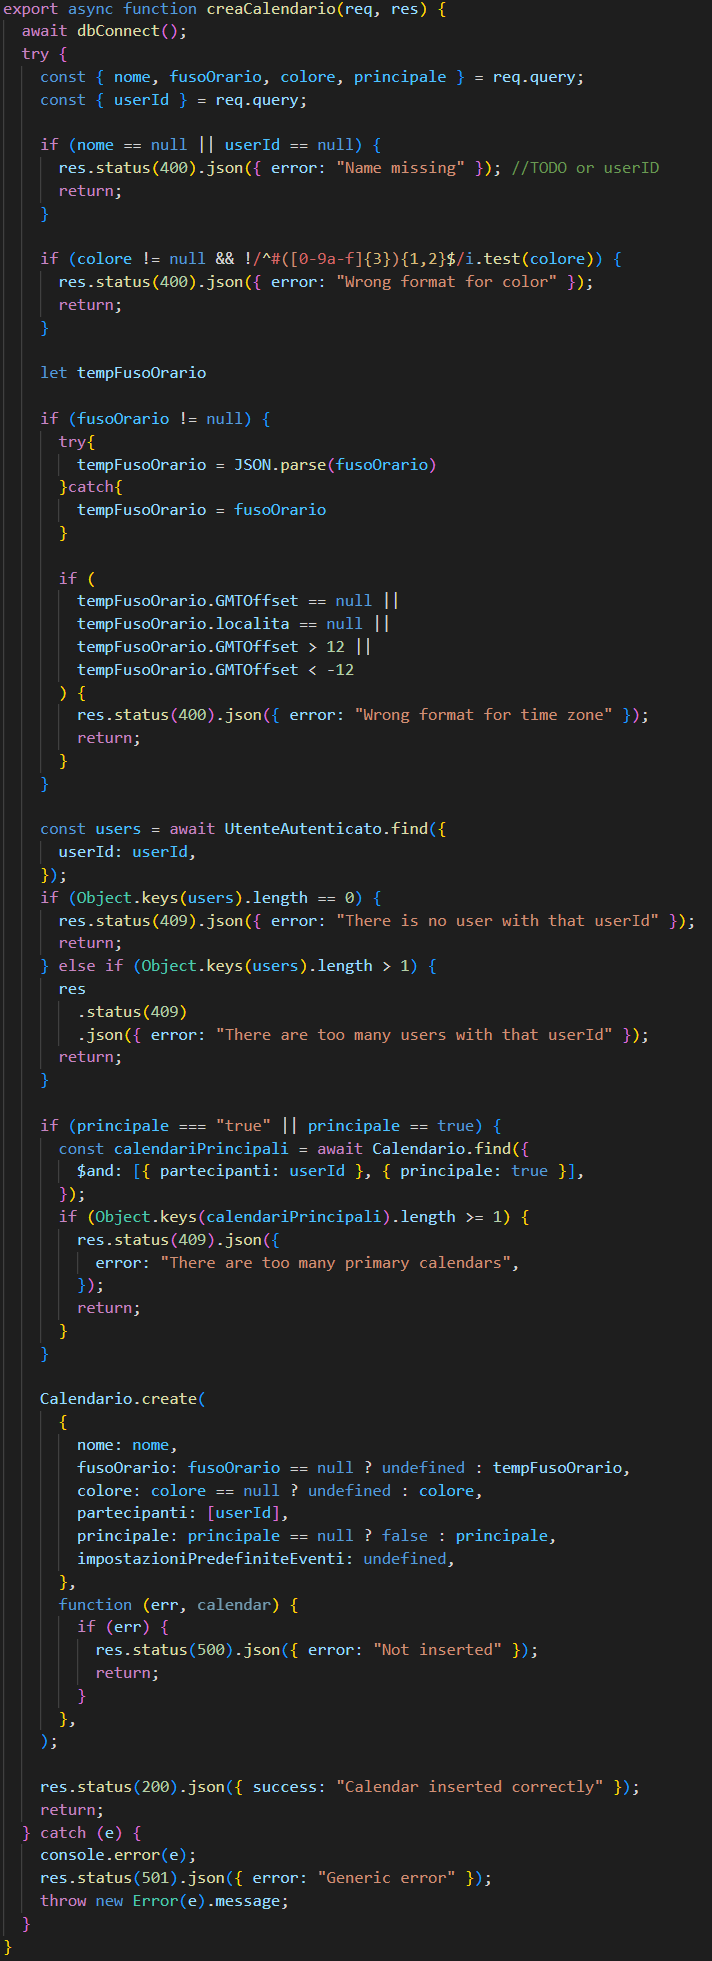
\includegraphics[width=0.55\textwidth, height=0.80\textheight]{img/png/APIs/creaCalendario.png}
                    \captionof{figure}{API - creaCalendario}
                    \blfootnote{Immagine \href{https://github.com/Life-planner/Documentazione/blob/main/D4/img/png/APIs/creaCalendario.png}{PNG} API - creaCalendario}
                \end{center}
                \begin{center}
                    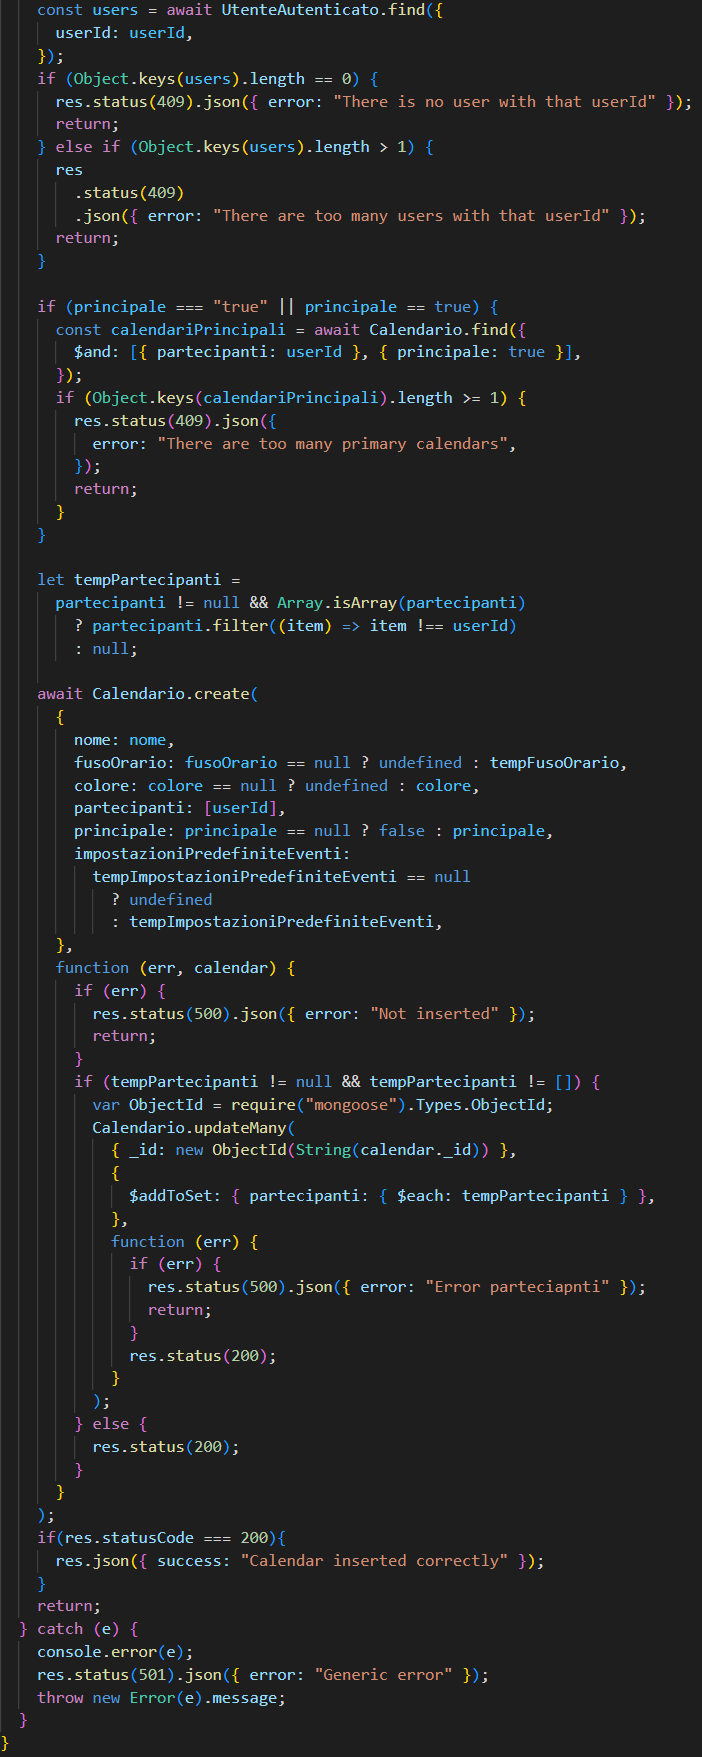
\includegraphics[width=0.55\textwidth, height=0.85\textheight]{img/png/APIs/creaCalendario2.png}
                    \captionof{figure}{API - creaCalendario, 2a parte}
                    \blfootnote{Immagine \href{https://github.com/Life-planner/Documentazione/blob/main/D4/img/png/APIs/creaCalendario2.png}{PNG} API - creaCalendario, 2a parte}
                \end{center}
                \newpage
        \elemento [Modifica Calendario] {apd:modificaCalendario}
                Grazie a questa API, già mostrata in parte in \ref{apd:ResourcesModelCalendario}, PlanIt riesce a modificare le impostazioni di un calendario già salvato per un utente autenticato. Per fare tale operazione, oltre all' "IDCalendario", "id" del calendario che si vuole modificare, e l' "userId", "id" dell'utente autenticato che vuole modificare un proprio calendario, sono necessari anche tutti gli altri attributi che costituiscono la struttura dati "Calendario", già molte volte mostrata come in (\ref{apd:ProjectDB}), con i quali si andrà a modificare il calendario. Nel caso in cui mancasse uno di questi attributi, si riceve il messaggio di errore: "400 - Parameter missing". \\
                Come si può notare dal codice, in "modificaCalendario" sono presenti gli stessi controlli già descritti in "creaCalendario", ma con l'aggiunta di qualcuno di nuovo. Infatti per l'oggetto "impostazioniPredefiniteEventi", che ricordiamo essere l'insieme di valori con cui vengono precompilati gli eventi appartenenti ad un calendario specifico, valori che possono essere modificati sia durante la creazione che modifica di un evento in fase di compilazione, vengono fatti ulteriori accertamenti. In primo luogo, vengono controllati che ciascun campo che lo forma sia diverso da "null", inoltre:
                \begin{itemize}
                    \item la "latitudine" e "longitudine" devono avere dei valori coerenti con la realtà (la longitudine deve essere nell'intervallo [-180,+180], invece la latitudine [-90,+90]);
                    \item la "priorità" e "difficoltà" devono avere un valore tra 0 e 10;
                    \item la "durata" deve essere maggiore di 0;
                    \item "tempAnticNotifica", attributo che indica quanto prima inviare la notifica di un evento, deve essere maggiore e uguale a 0.
                \end{itemize}
                Nel caso in cui una delle restrizioni sopra citate non fossero rispettate per "impostazioniPredefiniteEventi", si riceverebbe il messaggio di errore "400 - Wrong format impostazioni predefinite". \\
                Un altro controllo che viene fatto, è se il calendario, che si vuole modificare, appartenga o meno alla lista di calendari di quell'utente autenticato identificato dall' "userId". Questo controllo viene fatto grazie alla funzione "find()" che va a trovare nel database il calendario con l' "IDCalendario" inserito, e dopo aver ottenuto questo oggetto, viene controllato che il suo proprietario (primo utente presente nella lista di partecipanti al calendario, attributo che indica chi partecipa ad un calendario, ovvero ai suoi eventi) sia uguale all' "userId" inserito in input. Nel caso non lo fosse, si riceve il messaggio di errore: "409 - You do not own the calendar". \\
                Infine, invece che usare la funzione "create()", usata per salvare un calendario nel database in "creaCalendario", viene usata la funzione "updataMany()" che va ad aggiornare gli attributi che costituiscono il calendario che si vuole modificare secondo i parametri ricevuti in input.
                \begin{center}
                    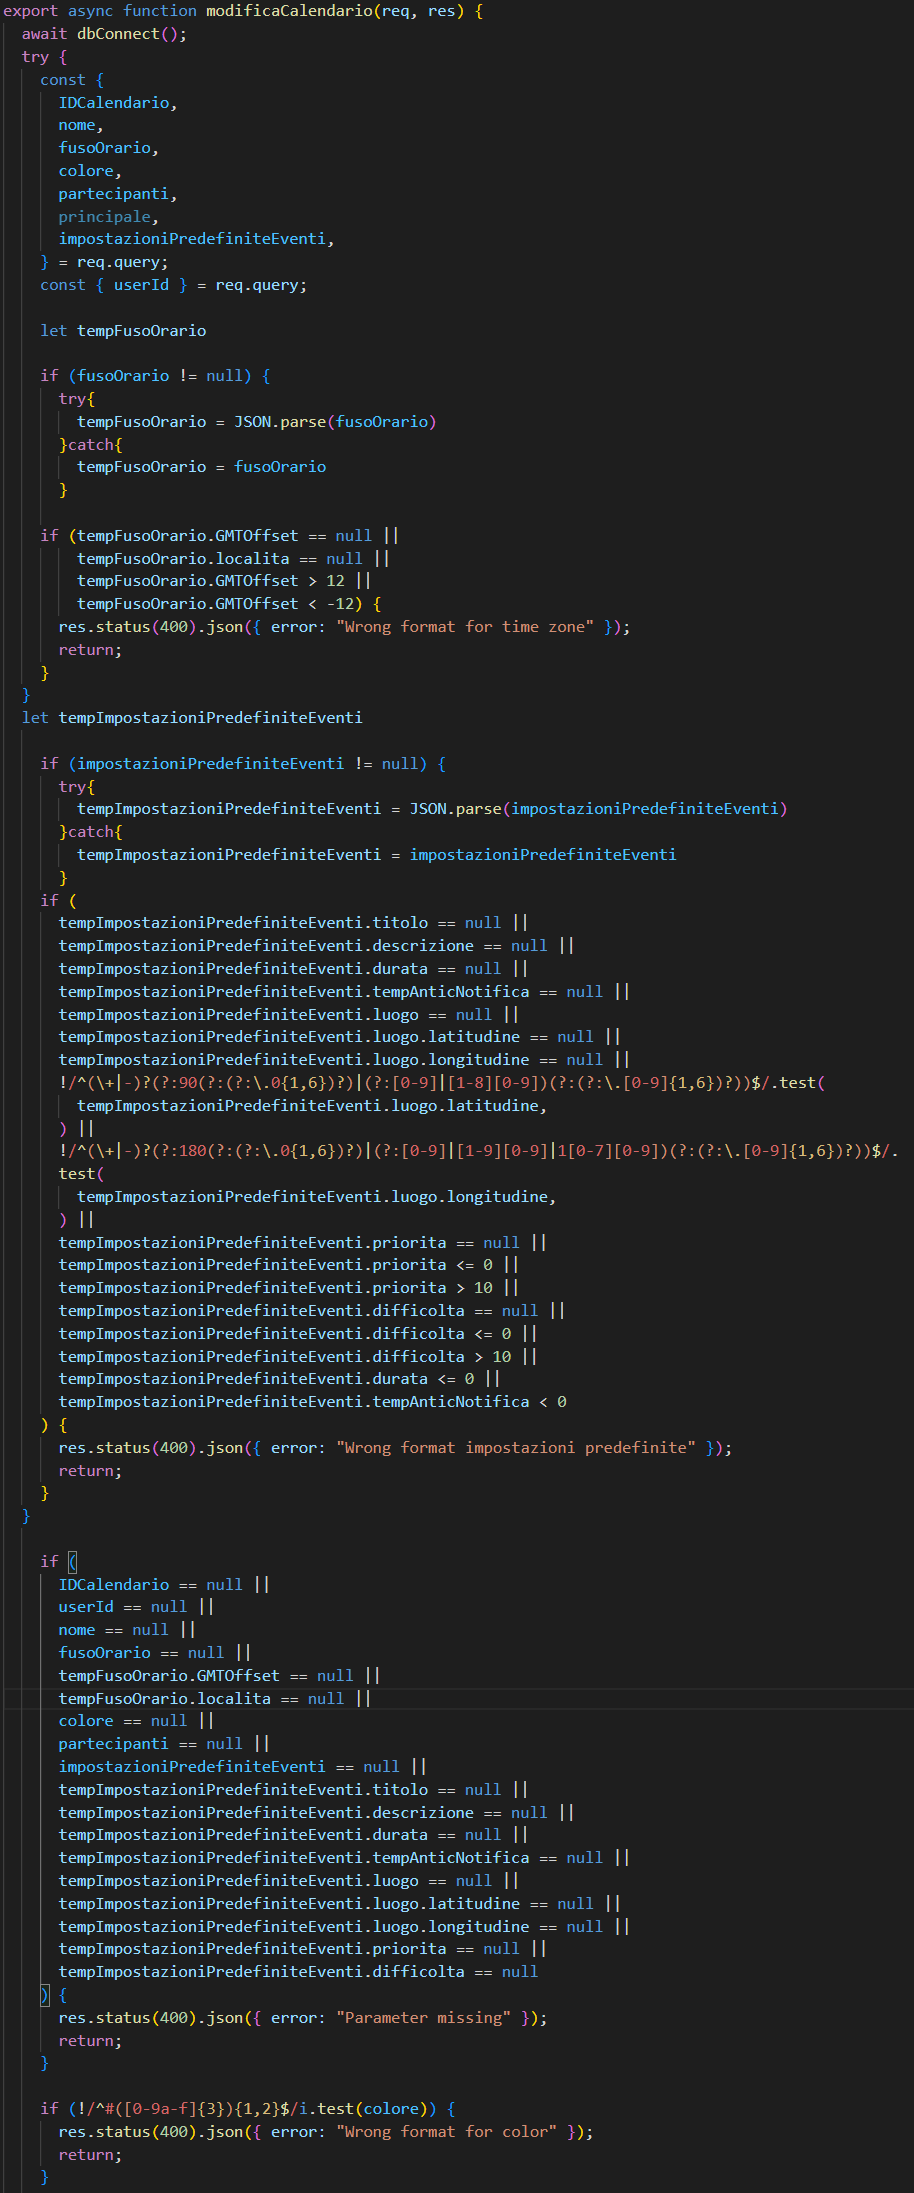
\includegraphics[width=0.6\textwidth, height=0.9\textheight]{img/png/APIs/modificaCalendario.png}
                    \captionof{figure}{API - modificaCalendario, 1a parte}
                    \blfootnote{Immagine \href{https://github.com/Life-planner/Documentazione/blob/main/D4/img/png/APIs/modificaCalendario.png}{PNG} API - modificaCalendario}
                \end{center}
                \begin{center}
                    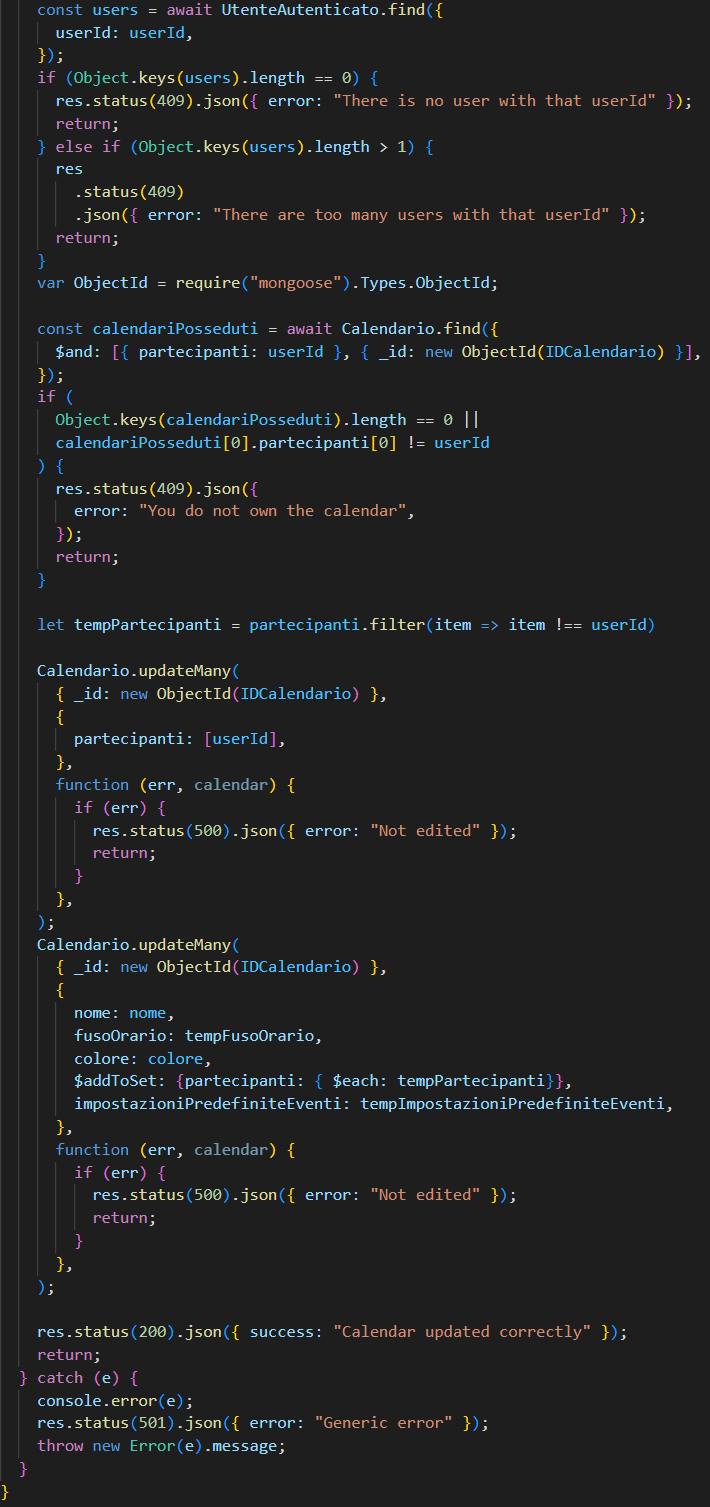
\includegraphics[width=0.6\textwidth, height=0.75\textheight]{img/png/APIs/modificaCalendario2.png}
                    \captionof{figure}{API - modificaCalendario, 2a parte}
                    \blfootnote{Immagine \href{https://github.com/Life-planner/Documentazione/blob/main/D4/img/png/APIs/modificaCalendario2.png}{PNG} API - modificaCalendario, 2a parte}
                \end{center}
        \elemento [Elimina Calendario] {apd:eliminaCalendario}
                Lo scopo di questa API, come già descritto in \ref{apd:ResourcesModelCalendario}, è quella di eliminare un calendario, dato il suo "IDCalendario" e l' "userId", per questo motivo questi due parametri non devono essere vuoti, sennò si riceve il messaggio di errore "400 - Parameter missing". Anche in questa API, come in "modificaCalendario" (\ref{apd:modificaCalendario}), viene controllato che l' "userId" inviato non sia un duplicato, che esista, che il calendario che si vuole eliminare appartenga alla lista di calendari dell'utente autenticato identificato dall' "userId". \\
                Infine, per eliminare il calendario dal database viene usata la funzione "deleteMany()" che sfrutta solo l' "IDCalendario" inviato in input per identificare il calendario da eliminare. Nel caso in cui non fosse eliminato nessun calendario per qualche motivo, c'è l'invio dell'errore "500 - Calendar not deleted"; un motivo che porta questo errore è la sconnessione improvvisa dal database MongoDB.
                \begin{center}
                    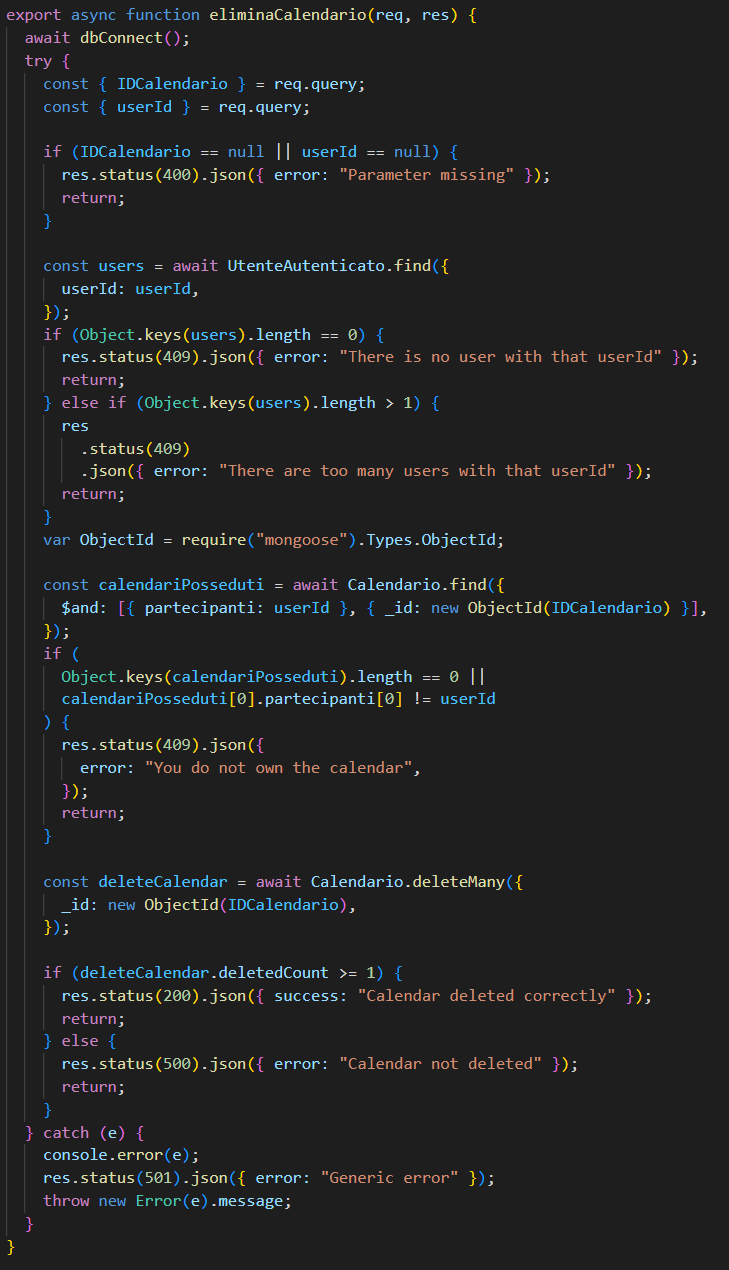
\includegraphics[width=0.8\textwidth, height=0.9\textheight]{img/png/APIs/eliminaCalendario.png}
                    \captionof{figure}{API - eliminaCalendario}
                    \blfootnote{Immagine \href{https://github.com/Life-planner/Documentazione/blob/main/D4/img/png/APIs/eliminaCalendario.png}{PNG} API - eliminaCalendario}
                \end{center}
        \elemento [getCalendari] {apd:getCalendari}
                L'applicativo PlanIt usa questa API, come già detto in \ref{apd:ResourcesModelCalendario}, per ottenere tutti i calendari dell'utente autenticato identificato dall' "userId" ricevuto in input. Dunque l'unico parametro che deve essere presente, per non riceve l'errore "400 - Parameter missing", è l' "userId", su cui si fanno sempre i soliti controlli. Alla fine della procedura, se questa va a buon fine, si ottiene l'array di strutture dati "Calendario" (già mostrata in \ref{apd:ProjectDB}) che appartengono all' utente autenticato che ha tale "userId".
                \begin{center}
                    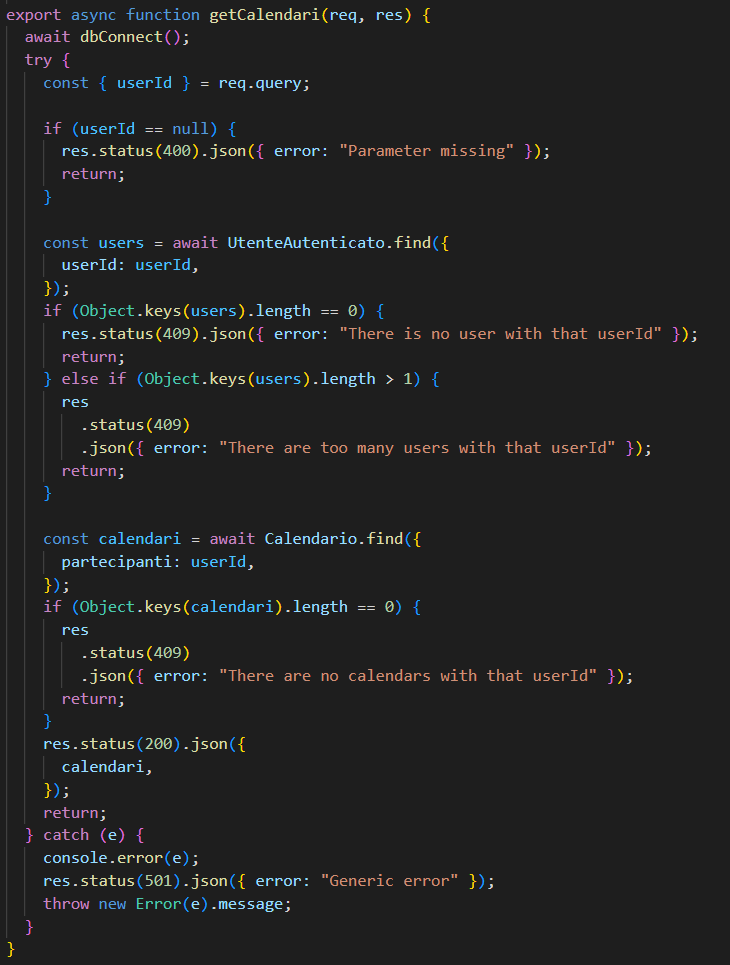
\includegraphics[width=0.65\textwidth, height=0.55\textheight]{img/png/APIs/getCalendari.png}
                    \captionof{figure}{API - getCalendari}
                    \blfootnote{Immagine \href{https://github.com/Life-planner/Documentazione/blob/main/D4/img/png/APIs/getCalendari.png}{PNG} API - getCalendari}
                \end{center}
                \newpage
        \elemento [Crea Evento] {apd:creaEvento}
                Mediante questa API, l'applicativo PlanIt riesce a salvare nel database MongoDB un evento con gli attributi uguali ai parametri inviati in input, per l'utente autenticato identificato dall' "userId" indicato. Già in \ref{apd:ResourcesModelEvento}, nella descrizione della risorsa "Crea Evento", siamo andati a presentare quali sono i casi in cui questa API invia come messaggio di errore "400 - IDCalendario or titolo or evento details missing", per questo motivo non andremo a ripeterli nuovamente. \\
                Come si può notare per gli attributi "luogo", "prorita", "difficolta", "notifiche" e "durata" vengono fatti gli stessi controlli già presentati in "modificaCalendario" (\ref{apd:modificaCalendario}) per l'attributo "impostazioniPredefiniteEventi", in quanto quest'ultimo oggetto contiene gli attributi sopra citati, presenti anche durante la crazione e modifica di un evento, dunque non vengono riscritti tutti specificamente. Nel caso in cui uno di questi attributi non passasse un controllo, riceviamo un errore del tipo "400 - Wrong format (parameter)". \\
                I controlli non presenti nelle altre API già descritte, riguardano gli attributi "eventoSingolo" ed "eventoRipetuto", oggetti che contengono informazioni fondamentali per creare un evento singolo, evento che poniamo solo in un giorno in fase di creazione, e un evento ripetuto, evento che poniamo su più giornate in fase di creazione o modifica. Per la struttura dati "eventoSingolo" andiamo a controllare che gli attributi "data" e "isScadenza" (questo attributo indica se l'evento che si sta mettendo con tale data sia una deadline di qualcosa oppure no) siano diversi da "null": se lo fossero riceviamo il messaggio di errore "400 - Wrong format for eventoSingolo".  Invece, per la struttura dati "eventoRipetuto" andiamo ad controllare che "numeroRipetizione", attributo che indica quante volte si ripete tale evento, sia diverso da "null" e maggiore e uguale di 1, che "data", attributo che indica il giorno, mese, anno e orario dell'evento, sia diverso da "null" e che, infine, "giornidellaSettimana", attributo che indica in quali giorni si ripete tale evento, sia diverso da "null" e che non sia un array vuoto. Se questi attributi non rispettassero queste restrizioni, riceviamo l'errore "400 - Wrong format for eventoRipetuto". \\
                Dopo sono presenti i soliti controlli già citati per il parametro "userId", ma evidenziamo la presenza della funzione "find()" che viene utilizzata per andare a vedere se il calendario, dove stiamo aggiungendo l'evento da che si sta creando, esista e appartenga all'utente autenticato identificato dall' "userId"; se così non fosse, otteniamo il messaggio di errore  "409 - There is no calendar with that ID or you do not own the calendar". Come per "creaCalendario" (\ref{apd:creaCalendario}), viene usata la funzione "create()" per andare a creare nel database MongoDB un oggetto "Evento" con le caratteristiche dei parametri ricevuti in input.
                \begin{center}
                    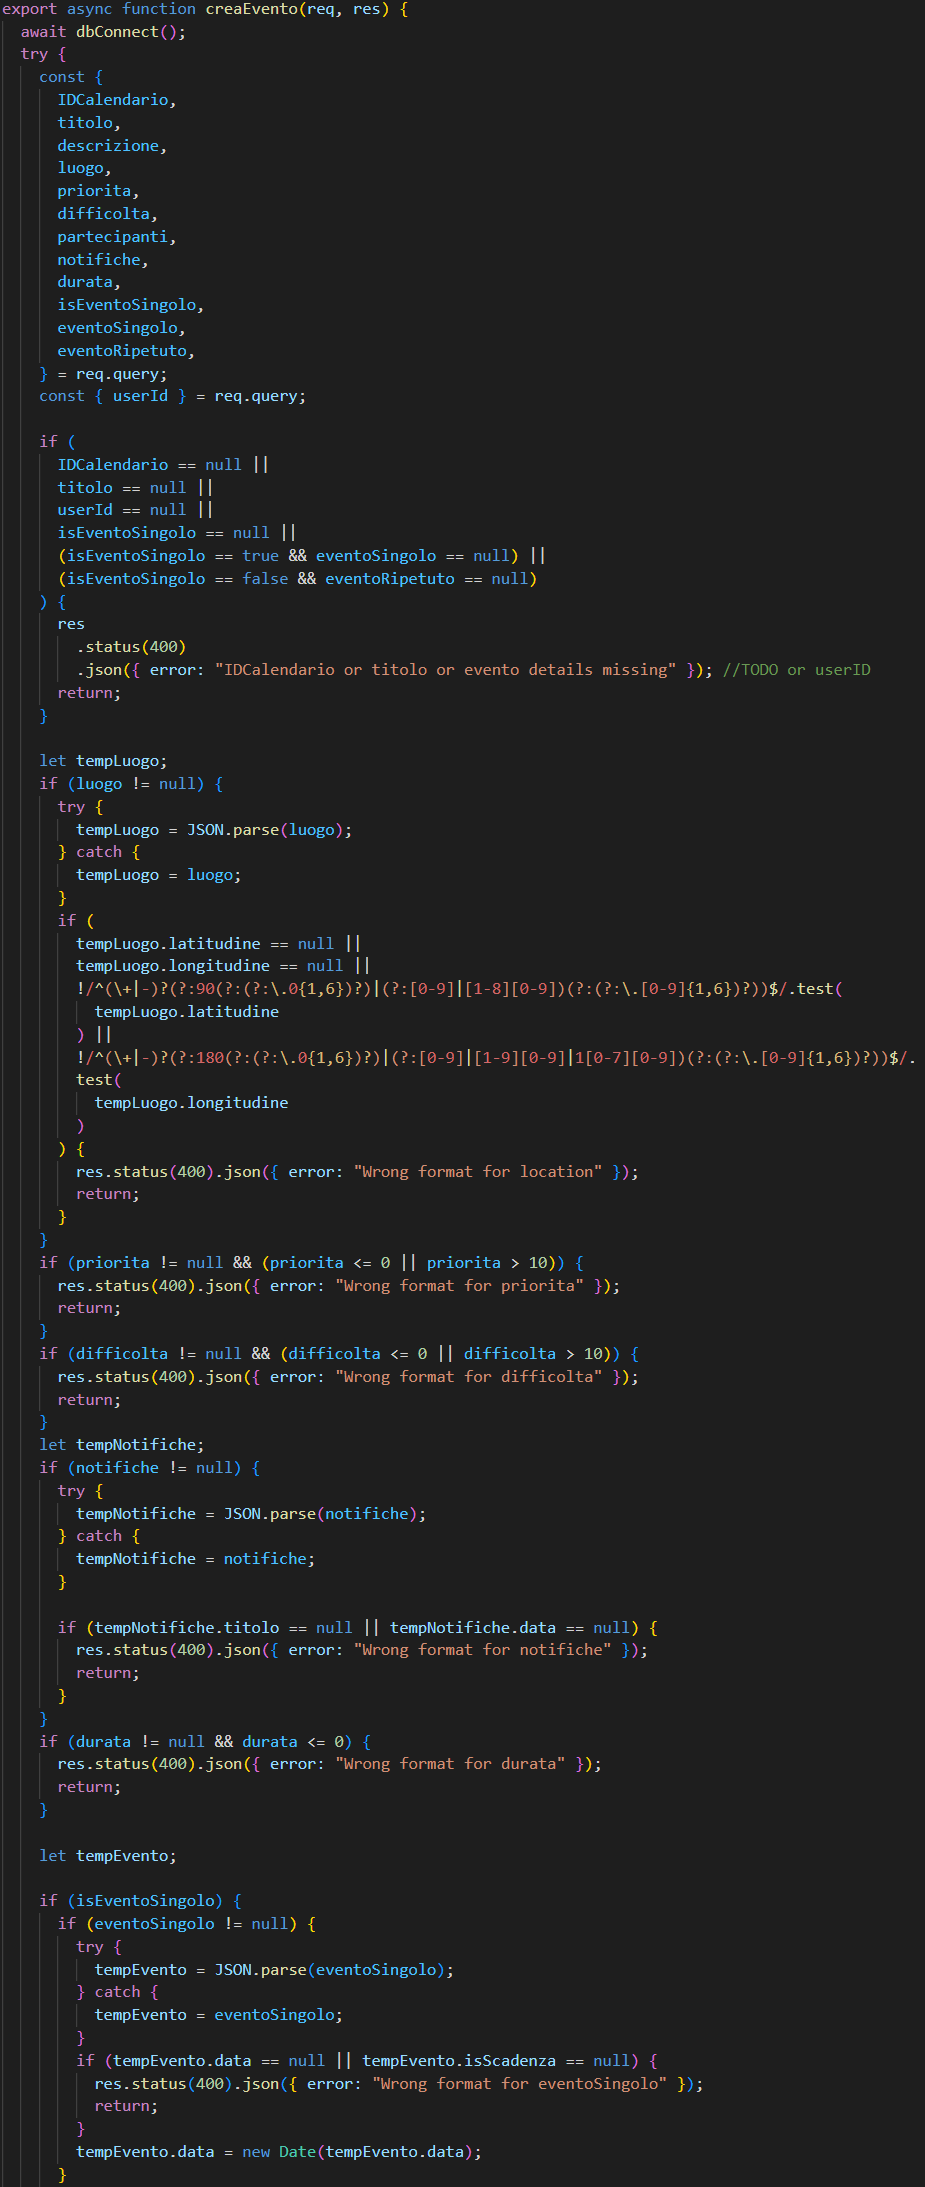
\includegraphics[width=0.55\textwidth, height=0.9\textheight]{img/png/APIs/creaEvento.png}
                    \captionof{figure}{API - creaEvento, 1a parte}
                    \blfootnote{Immagine \href{https://github.com/Life-planner/Documentazione/blob/main/D4/img/png/APIs/creaEvento.png}{PNG} API - creaEvento, 1a parte}
                \end{center}
                \begin{center}
                    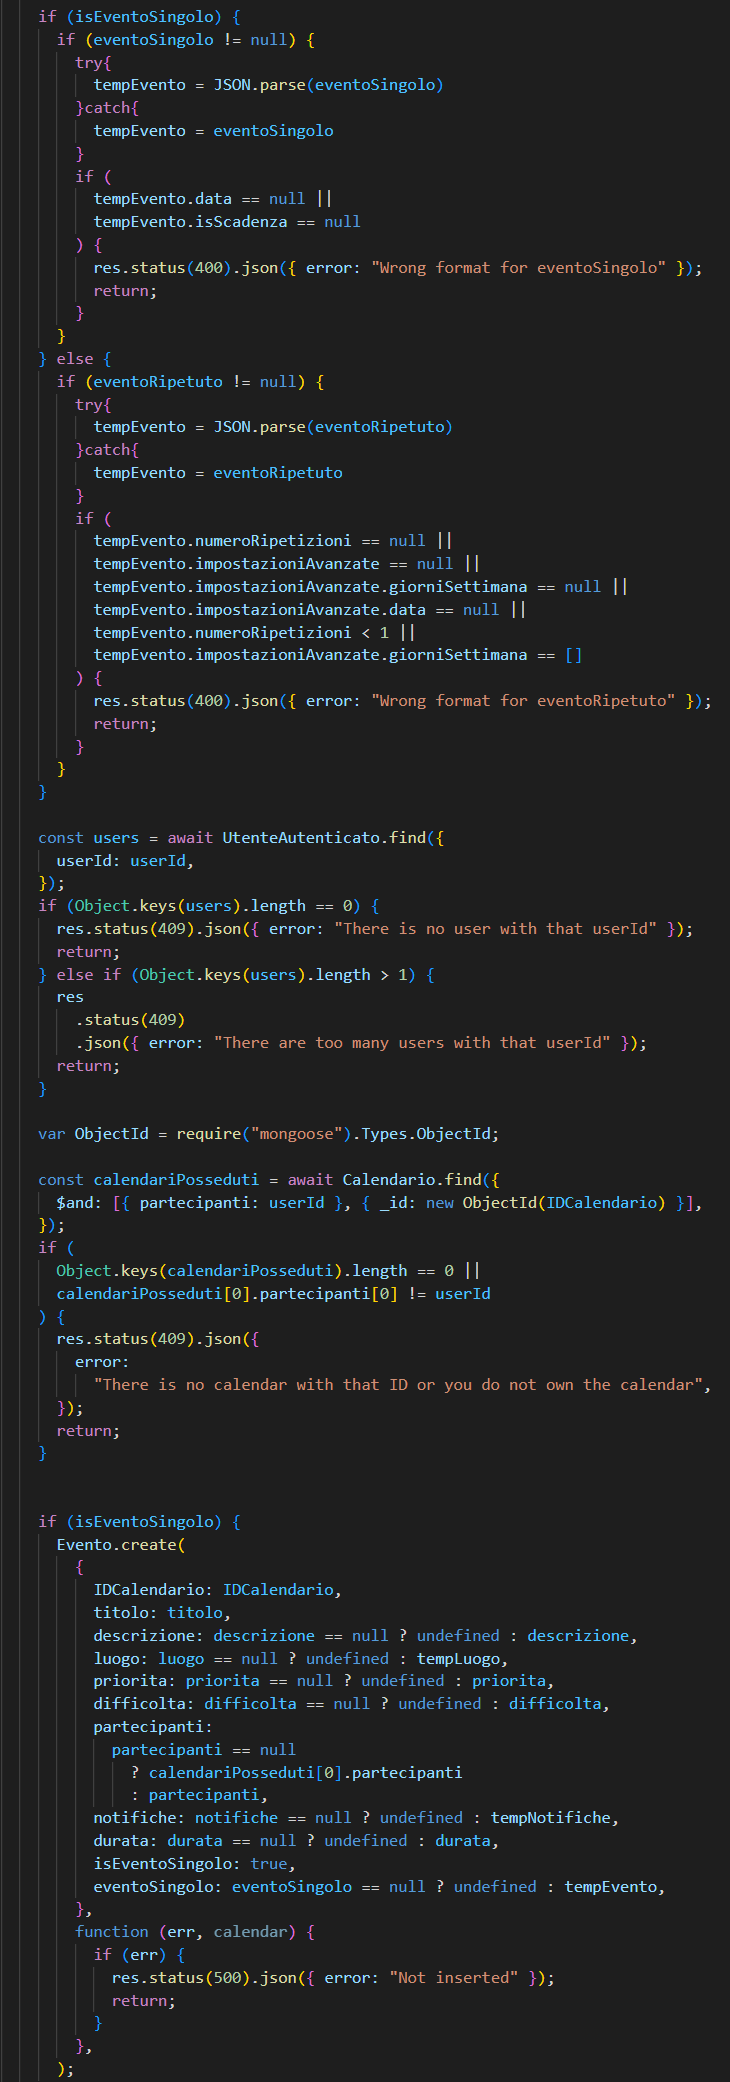
\includegraphics[width=0.5\textwidth, height=0.9\textheight]{img/png/APIs/creaEvento2.png}
                    \captionof{figure}{API - creaEvento, 2a parte}
                    \blfootnote{Immagine \href{https://github.com/Life-planner/Documentazione/blob/main/D4/img/png/APIs/creaEvento2.png}{PNG} API - creaEvento, 2a parte}
                \end{center}
                \begin{center}
                    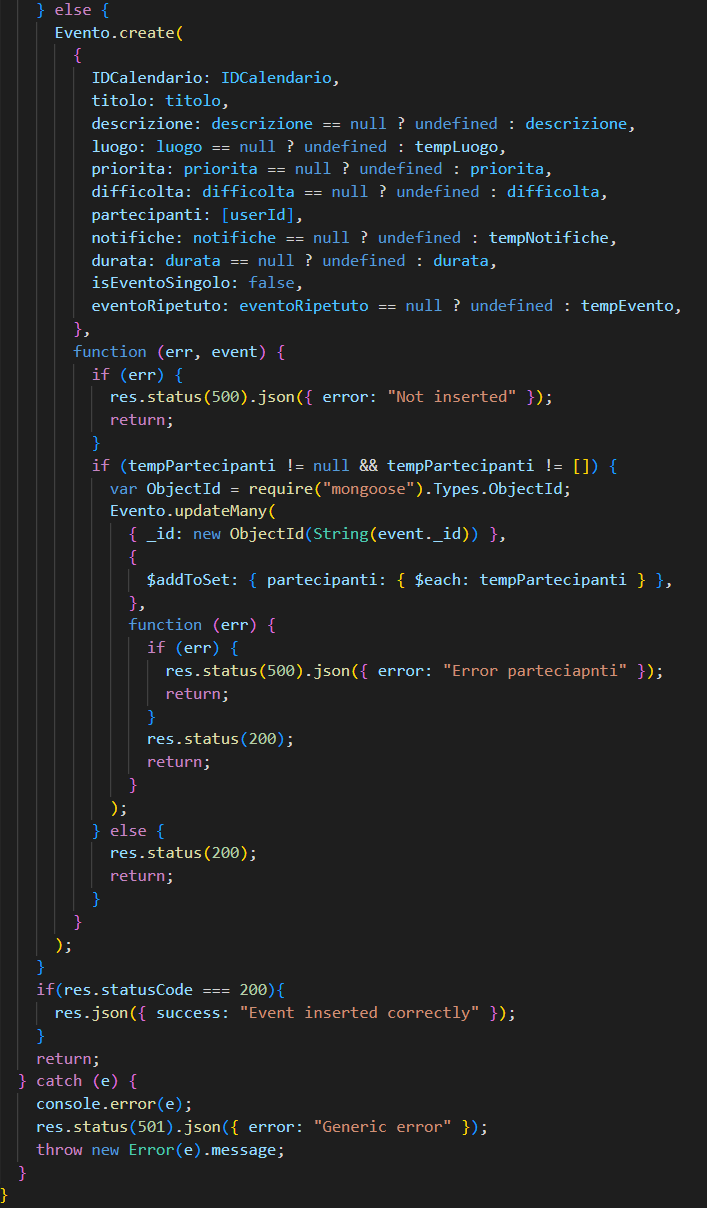
\includegraphics[width=0.75\textwidth, height=0.9\textheight]{img/png/APIs/creaEvento3.png}
                    \captionof{figure}{API - creaEvento, 3a parte}
                    \blfootnote{Immagine \href{https://github.com/Life-planner/Documentazione/blob/main/D4/img/png/APIs/creaEvento3.png}{PNG} API - creaEvento, 3a parte}
                \end{center}
        \elemento [Modifica Evento] {apd:modificaEvento}
                Grazie a questa API, come già detto in \ref{apd:ResourcesModelEvento}, è possibile modificare un "Evento" già salvato nel database MongoDB, con i vari parametri ricevuti in input, che non sono altro che gli attributi che formano la struttura dati "Evento", struttura dati già più volte mostrata (\ref{apd:ProjectDB}), e l' "userId" dell'utente autenticato che vuole modificare tale evento. I controlli, presenti in questa API, sono gli stessi già descritti per "creaEvento" (\ref{apd:creaEvento}) e "modificaCalendario" (\ref{apd:modificaCalendario}); l'unica differenza è che per non ricevere il messaggio di errore "400 - Parameter missing", tutti gli attributi che andranno a formare l'oggetto "Evento" (\ref{apd:ProjectDB}) e l' "userId" devono essere diversi da "null". \\
                Alla fine della funzione, grazie alla funzione "updateMany()", viene aggiornato l'oggetto "Evento" presente nel database secondo i parametri ricevuti, come per "modificaCalendario" (\ref{apd:modificaCalendario}). Specifichiamo che a seconda se stiamo andando a modificare un "eventoSingolo" o "eventoRipetuto" abbiamo una diversa procedura di aggiornamento.
                \begin{center}
                    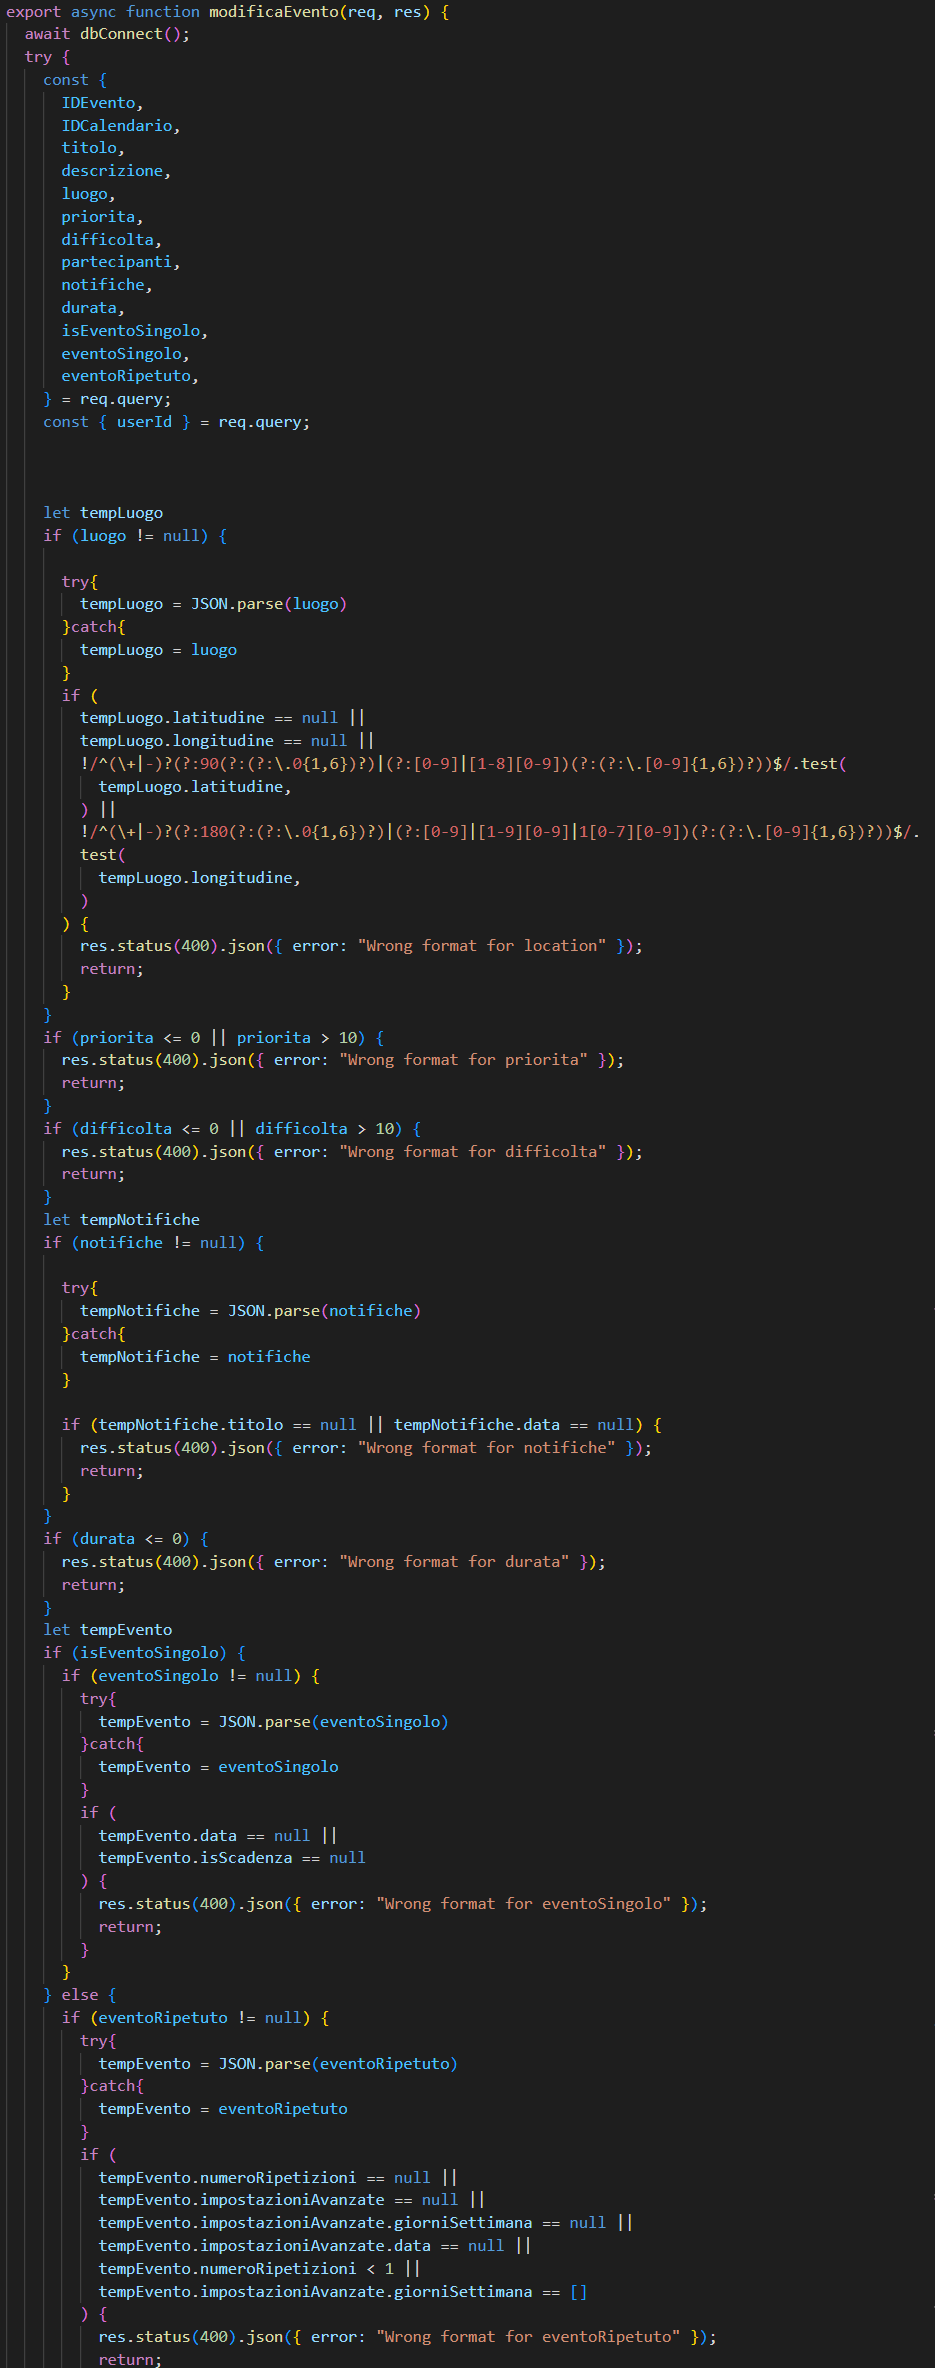
\includegraphics[width=0.55\textwidth, height=0.9\textheight]{img/png/APIs/modificaEvento.png}
                    \captionof{figure}{API - modificaEvento, 1a parte}
                    \blfootnote{Immagine \href{https://github.com/Life-planner/Documentazione/blob/main/D4/img/png/APIs/modificaEvento.png}{PNG} API - modificaEvento, 1a parte}
                \end{center}
                \begin{center}
                    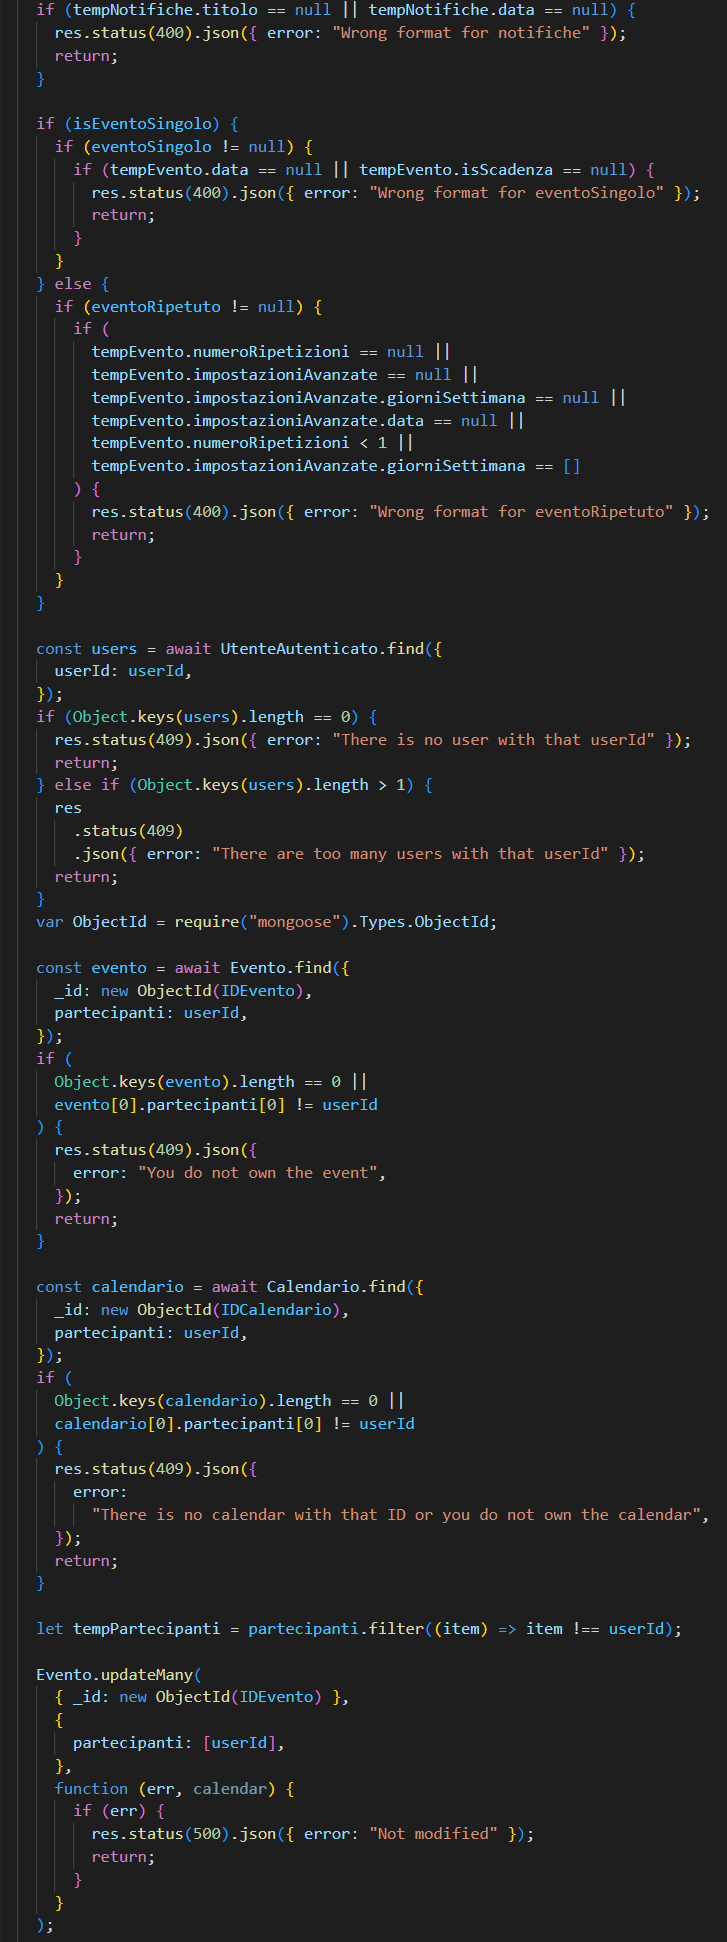
\includegraphics[width=0.45\textwidth, height=0.9\textheight]{img/png/APIs/modificaEvento2.png}
                    \captionof{figure}{API - modificaEvento, 2a parte}
                    \blfootnote{Immagine \href{https://github.com/Life-planner/Documentazione/blob/main/D4/img/png/APIs/modificaEvento2.png}{PNG} API - modificaEvento, 2a parte}
                \end{center}
                \begin{center}
                    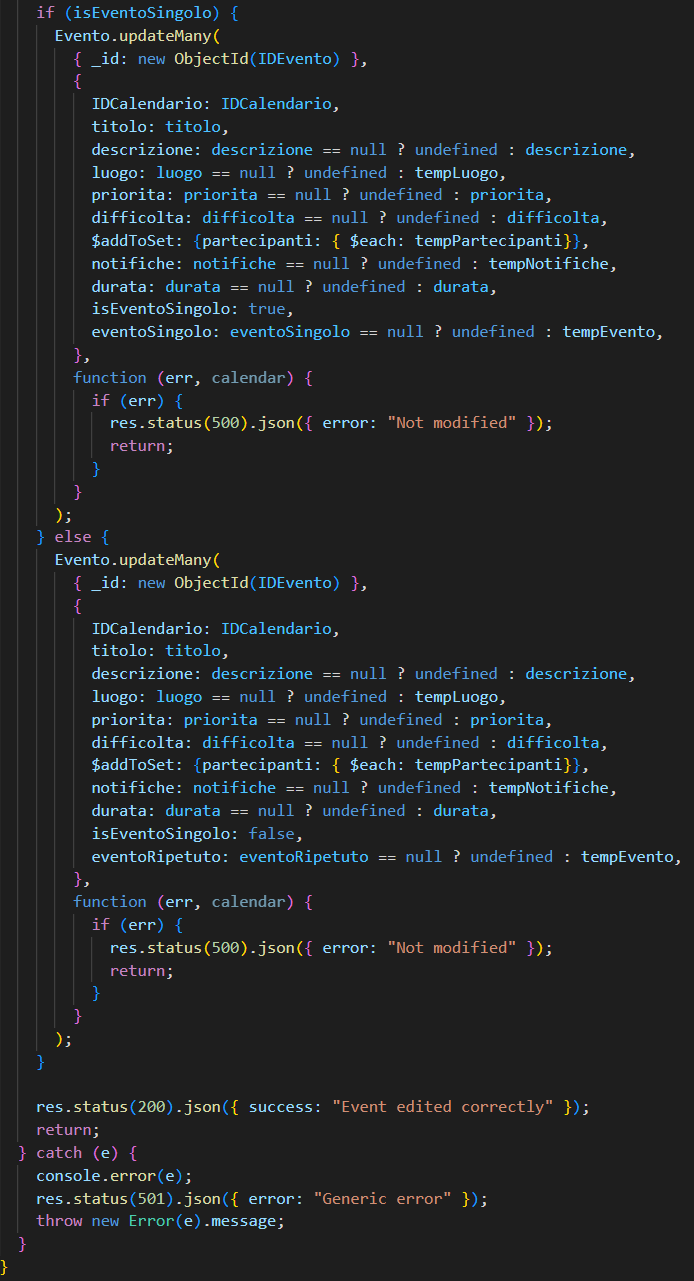
\includegraphics[width=0.55\textwidth, height=0.6\textheight]{img/png/APIs/modificaEvento3.png}
                    \captionof{figure}{API - modificaEvento, 3a parte}
                    \blfootnote{Immagine \href{https://github.com/Life-planner/Documentazione/blob/main/D4/img/png/APIs/modificaEvento2.png}{PNG} API - modificaEvento, 3a parte}
                \end{center}
        \elemento [Elimina Evento] {apd:eliminaEvento}
                Questa API, come già anticipato in \ref{apd:ResourcesModelEvento}, ha lo scopo di andare ad eliminare un "Evento", dato il suo "IDEvento" e l' "userId" dell'utente autenticato che ha questo evento che vuole eliminare. Ovviamente, nel caso in cui non avessimo uno di questi due parametri, come già detto in \ref{apd:ResourcesModelEvento}, otteniamo un messaggio di errore del tipo "400 - Parameter missing". \\
                In seguito, vengono fatti sempre gli stessi controlli già citati in "EliminaCalendario" \ref{apd:eliminaCalendario}, ma stavolta per gli eventi. Infatti si controlla che l'evento che si vuole eliminare faccia parte della lista degli eventi appartenenti all'utente autenticato indicato dall' "userId". Se così non fosse, l'API invia l'errore "409 - You do not own the event". \\
                Infine, anche per questa funzione vengono usate le funzioni "find()" e "deleteMany()" per ottenere rispettivamente la lista di eventi di un utente autenticato e per eliminare l'evento identificato dall' "IDEvento".
                \begin{center}
                    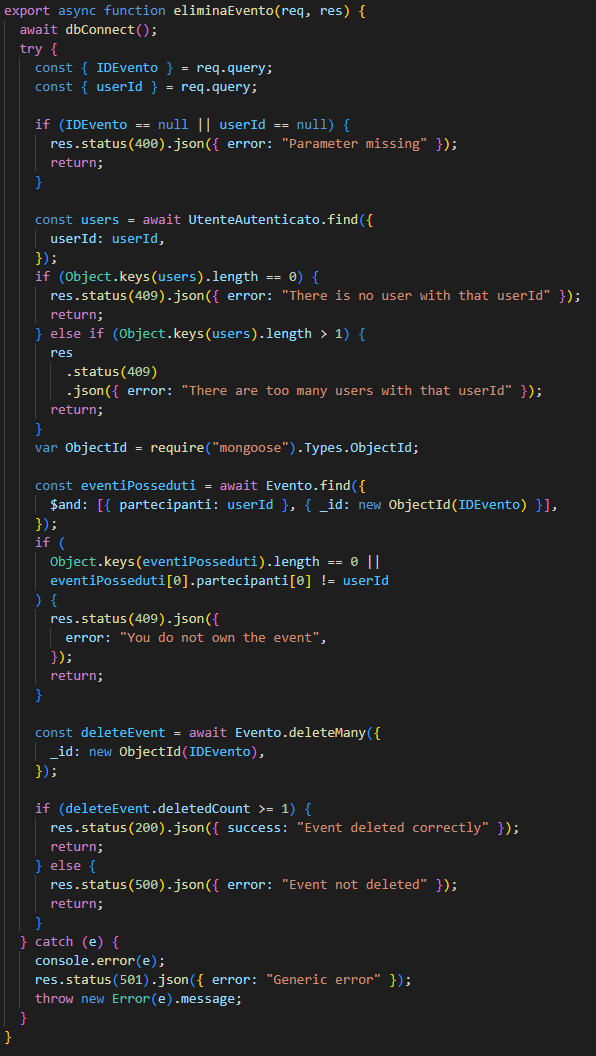
\includegraphics[width=0.65\textwidth, height=0.7\textheight]{img/png/APIs/eliminaEvento.png}
                    \captionof{figure}{API - eliminaEvento}
                    \blfootnote{Immagine \href{https://github.com/Life-planner/Documentazione/blob/main/D4/img/png/APIs/eliminaEvento.png}{PNG} API - eliminaEvento}
                \end{center}
                \newpage
        \elemento [getEventi] {apd:getEventi}
                Questa API, precedentemente descritta in \ref{apd:ResourcesModelEvento}, viene usata per ottenere tutti gli eventi che appartengono ad un calendario di un utente autenticato. Questo calendario viene identificato dall' "IDCalendario" e l' "userId" ricevuti in input, i quali, per ottenere un successo dalla procedura dell'API, non devono essere vuoti. Sul parametro "userId" vengono fatti i soliti controlli già presenti nelle altre API. Invece, dato l' "IDCalendario" e l' "userId", grazie alla funzione "find()", "getEventi" controlla che tale calendario esista e che appartenga alla lista dei calendari dell'utente autenticato; se così non si fosse, si riceve il messaggio di errore "409 - There is no calendar with that ID or you are not part of it". \\
                Infine, si controlla anche che questo calendario non sia vuoto, ovvero che abbia almeno un evento, in caso lo fosse si ottiene il messaggio di errore "409 - There are no events with that userId and IDCalendario", come già detto in \ref{apd:ResourcesModelEvento}.
                \begin{center}
                    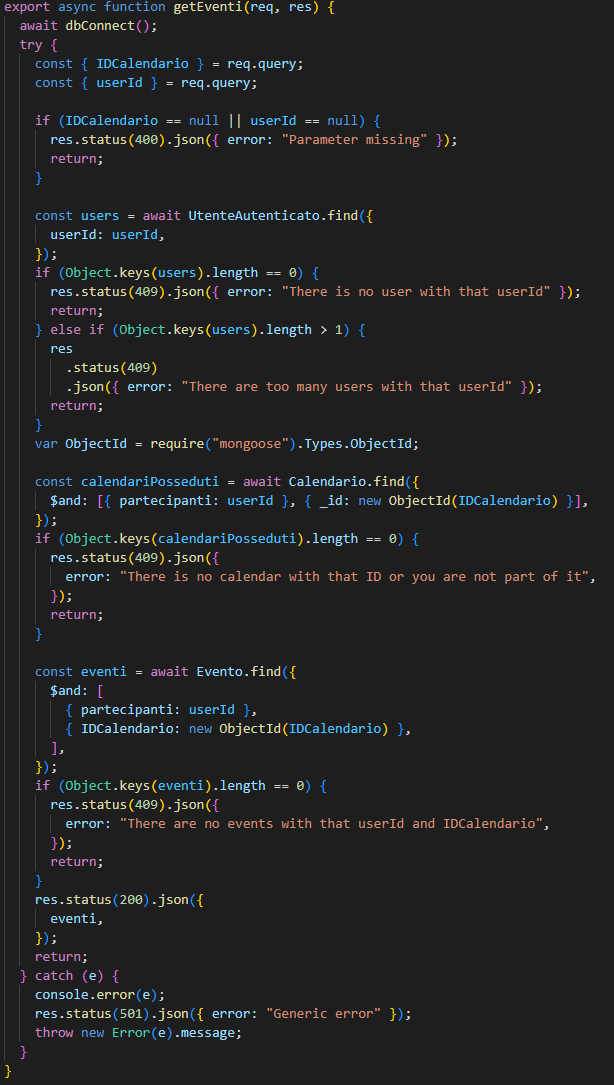
\includegraphics[width=0.60\textwidth, height=0.70\textheight]{img/png/APIs/getEventi.png}
                    \captionof{figure}{API - getEventi}
                    \blfootnote{Immagine \href{https://github.com/Life-planner/Documentazione/blob/main/D4/img/png/APIs/getEventi.png}{PNG} API - getEventi}
                \end{center}
        \elemento [Crea Account] {apd:creaAccount}
                Questa API (descritta in parte in \ref{apd:ResourcesModelUtenteAutenticato}) viene utilizzata per creare un "account", ovvero un oggetto di tipo "UtenteAutenticato", struttura dati già mostrata in precendenza in \ref{apd:ProjectDB}, all'interno del database MongoDB, la prima volta che un utente accede autenticandosi nel sito PlanIt. I parametri, che devono essere presenti per non ottenere il messaggio di errore "400 - Parameter missing", sono: "userId", "email" e "username" dell'utente autenticato che si vuole creare. \\
                I controlli che vengono effettuati sono gli stessi già descritti nelle altre API, si evidenzia la presenza della funzione "find()" che ha lo scopo di trovare se esistono nel database già utenti con l' "userId" o l' "email" inseriti in input; se ne esistessero otteniamo come errore "409 - There is already one user with that id or email". \\
                Alla fine della funzione, viene usata la funzione "create()" per andare a creare nel database un oggetto "UtenteAutenticato" con gli attributi ricevuti come parametri.
                \begin{center}
                    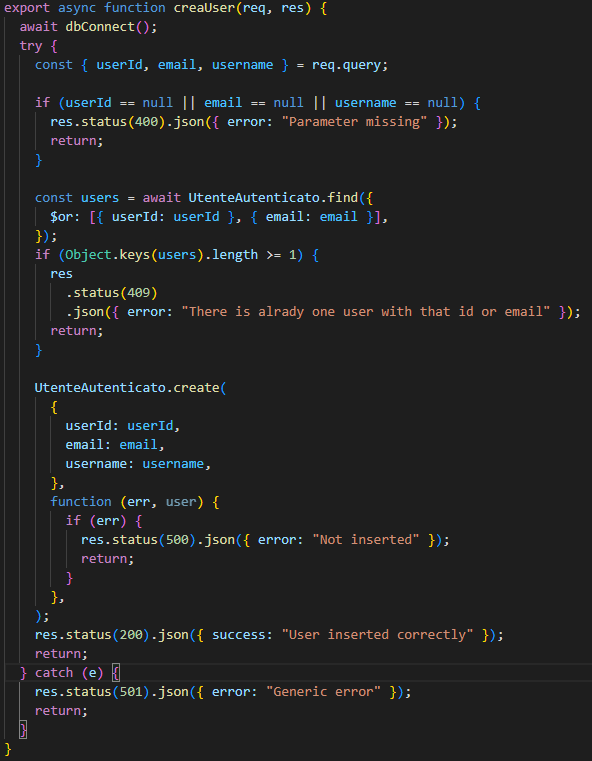
\includegraphics[width=0.65\textwidth, height=0.55\textheight]{img/png/APIs/creaUser.png}
                    \captionof{figure}{API - creaAccount}
                    \blfootnote{Immagine \href{https://github.com/Life-planner/Documentazione/blob/main/D4/img/png/APIs/creaUser.png}{PNG} API - creaAccount}
                \end{center}
                \newpage
        \elemento [Modifica Account] {apd:modificaAccount}
                L'applicativo PlanIt sfrutta questa API, già anticipata in parte in \ref{apd:ResourcesModelUtenteAutenticato}, per andare a modificare l'account, più precisamente l' "username", di un oggetto "UtenteAutenticato" già presente nel database. Per andare a modificare l'oggetto "UtenteAutenticato" vengono utilizzati i parametri che sono ricevuti in input, che non sono altro che gli attributi che formano un oggetto di tipo "UtenteAutenticato" (guardare \ref{apd:ProjectDB}). Per andare ad identificare l'utente da modificare viene usato l' "userId" ricevuto, invece l' "username" è l'attributo che viene modificato nell'oggetto "UtenteAutenticato" già presente nel database. I controlli effettuati, all'interno di questa API, sono gli stessi già descritti per altre API; infatti si controlla che l' "userId" inserito corrisponda ad un utente esistente e non duplicato e che la funzione "updateMany()" esegua con nessun tipo di errore.
                \begin{center}
                    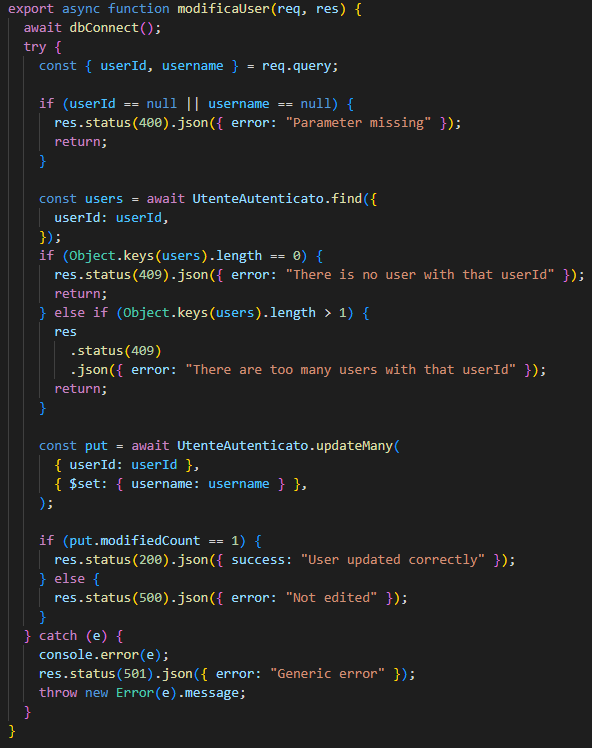
\includegraphics[width=0.65\textwidth, height=0.55\textheight]{img/png/APIs/modificaUser.png}
                    \captionof{figure}{API - modificaAccount}
                    \blfootnote{Immagine \href{https://github.com/Life-planner/Documentazione/blob/main/D4/img/png/APIs/modificaUser.png}{PNG} API - modificaAccount}
                \end{center}
                \newpage
        \elemento [Get Dati Account - userId] {apd:getDatiAccount_userId}
                Questa API viene utilizzata per ottenere in output un oggetto di tipo "UtenteAutenticato" che abbia l' "userId" uguale al parametro "userId" inserito in input. Nel caso in cui l' "userId" non fosse ricevuto in input o non corrispondesse a nessun "UtenteAutenticato" salvato nel database o corrispondesse a più utenti, riceviamo un messaggio di errore diverso per ciascuno dei casi, già descritti più volte precedentemente nelle altre APIs.
                \begin{center}
                    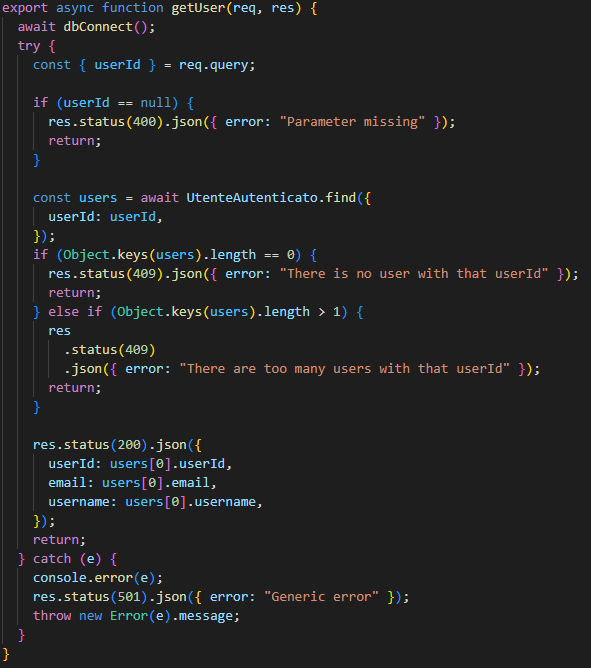
\includegraphics[width=0.65\textwidth, height=0.55\textheight]{img/png/APIs/getUser_userId.png}
                    \captionof{figure}{API - Get Dati Account\_userId}
                    \blfootnote{Immagine \href{https://github.com/Life-planner/Documentazione/blob/main/D4/img/png/APIs/getUser_userId.png}{PNG} API - Get Dati Account\_userId}
                \end{center}
                \newpage
        \elemento [Get Dati Account - email] {apd:getDatiAccount_email}
                Questa API viene utilizzata per ottenere in output un oggetto di tipo "UtenteAutenticato" che abbia l' "email" uguale al parametro "email" inserito in input. Questa API fa la stessa procedura e ha lo stesso scopo dell'API descritta in \ref{apd:getDatiAccount_userId}, ovvero quella precedente (Get Dati Account - userId), l'unica cosa che cambia è che viene utilizzata l'email per identificare univocamente un "UtenteAutenticato". Con entrambe le APIs, ad ogni modo, si dovrebbe ottenere lo stesso risultato in quanto sia l' "userId" che l' "email" dovrebbero identificare univocamente un "UtenteAutenticato".
                \begin{center}
                    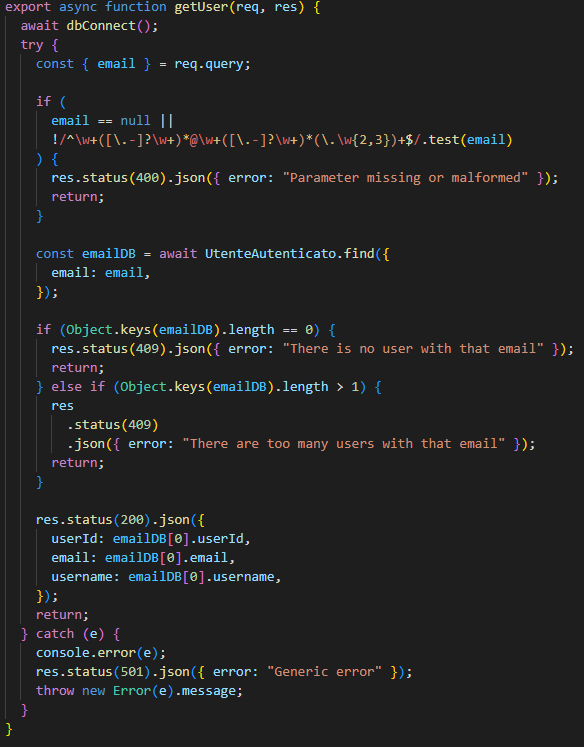
\includegraphics[width=0.65\textwidth, height=0.55\textheight]{img/png/APIs/getUser_email.png}
                    \captionof{figure}{API - Get Dati Account\_email}
                    \blfootnote{Immagine \href{https://github.com/Life-planner/Documentazione/blob/main/D4/img/png/APIs/getUser_email.png}{PNG} API - Get Dati Account\_email}
                \end{center}
                \newpage
    \end{listaPersonale2}
\end{listaPersonale}